\documentclass{article}[12pt]
\usepackage[utf8]{inputenc}
\usepackage[T1]{fontenc}
\usepackage[ngerman]{babel}

\usepackage[dvipsnames]{xcolor}
\usepackage{lipsum}

\usepackage{amsfonts}
\usepackage[intlimits]{amsmath}
\usepackage{cite}
\usepackage{epsfig}

\usepackage[usenames,dvipsnames]{pstricks}
\usepackage{pstricks-add}
\usepackage{epsfig}
\usepackage{pst-grad} % For gradients
\usepackage{pst-plot} % For axes

\addtolength{\hoffset}{-1.5cm}
\addtolength{\textwidth}{3cm}
\usepackage{listings}
\usepackage{color}
\definecolor{mygreen}{rgb}{0,0.6,0}
\definecolor{mygray}{rgb}{0.5,0.5,0.5}
\definecolor{mymauve}{rgb}{0.58,0,0.82}
\PassOptionsToPackage{svgnames}{xcolor}
\usepackage{tcolorbox}
\usepackage{lipsum}
\tcbuselibrary{skins,breakable}
\usetikzlibrary{shadings,shadows}

\lstset{ %
  backgroundcolor=\color{white},   % choose the background color; you must add \usepackage{color} or \usepackage{xcolor}; should come as last argument
  basicstyle=\footnotesize,        % the size of the fonts that are used for the code
  breakatwhitespace=false,         % sets if automatic breaks should only happen at whitespace
  breaklines=true,                 % sets automatic line breaking
  captionpos=b,                    % sets the caption-position to bottom
  commentstyle=\color{mygreen},    % comment style
  deletekeywords={...},            % if you want to delete keywords from the given language
  escapeinside={\%*}{*)},          % if you want to add LaTeX within your code
  extendedchars=true,              % lets you use non-ASCII characters; for 8-bits encodings only, does not work with UTF-8
  frame=single,	                   % adds a frame around the code
  keepspaces=true,                 % keeps spaces in text, useful for keeping indentation of code (possibly needs columns=flexible)
  keywordstyle=\color{blue},       % keyword style
  language=C,                      % the language of the code
  morekeywords={*,...},            % if you want to add more keywords to the set
  numbers=left,                    % where to put the line-numbers; possible values are (none, left, right)
  numbersep=5pt,                   % how far the line-numbers are from the code
  numberstyle=\tiny\color{mygray}, % the style that is used for the line-numbers
  rulecolor=\color{black},         % if not set, the frame-color may be changed on line-breaks within not-black text (e.g. comments (green here))
  showspaces=false,                % show spaces everywhere adding particular underscores; it overrides 'showstringspaces'
  showstringspaces=false,          % underline spaces within strings only
  showtabs=false,                  % show tabs within strings adding particular underscores
  stepnumber=1,                    % the step between two line-numbers. If it's 1, each line will be numbered
  stringstyle=\color{mymauve},     % string literal style
  tabsize=2,	                   % sets default tabsize to 2 spaces
  title=\lstname                   % show the filename of files included with \lstinputlisting; also try caption instead of title
}


\newenvironment{myexampleblock}[1]{%
    \tcolorbox[beamer,%
    noparskip,breakable,
    colback=White,colframe=ForestGreen,%
    colbacklower=LimeGreen!75!White,%
    title=#1]}%
    {\endtcolorbox}

\newenvironment{myalertblock}[1]{%
    \tcolorbox[beamer,%
    noparskip,breakable,
    colback=White,colframe=Bittersweet,%
    colbacklower=Peach!75!White,%
    title=#1]}%
    {\endtcolorbox}

\newenvironment{myblock}[1]{%
    \tcolorbox[beamer,%
    noparskip,breakable,
    colback=White,colframe=RoyalBlue,%
    colbacklower=TealBlue!75!White,%
    title=#1]}%
    {\endtcolorbox}

\newenvironment{myexampleprogram}[1]{%
    \tcolorbox[beamer,%
    noparskip,breakable,
    colback=White,colframe=Goldenrod,%
    colbacklower=Yellow!75!White,%
    title=#1]}%
    {\endtcolorbox}
%--------
%\usepackage[magyar]{babel}
\title{C Programmierkurs}
\begin{document}
\maketitle
\section{Einführung}
In diesem Kurz wir werden die C Programmier sprache kennenlernen. Programmierung besteht aus Code schreiben und die übersetztung dieser Code in
ausführbaren Maschinecode.
Es gibt Programmier Sprache, die jede Befehle nacheinander übersetzt und ausführt. C ist anders, hier die ganze Code muss zuerst schreiben und
kompiliert werden,  danach kann diene Programm ausführen. Wir nutzten Compiler unser Code zu Maschinencode zu übersetzten. Für ersten Programmier Sprache C ist ideal 
von mehreren Gründen:
\begin{itemize}
\item C ist sehr effizient
\item C hat high level konstrukte.
\end{itemize}
Es ist effizient, weil es sehr gute Compiler gibt. Wir müssen nicht die Teile des CPU-s wissen um eine gute Code zu schreiben, 
weil es high level konstrukte hat. Aber M\"oglicherweise das beste Antwort ist das C Kenntnisse ist unbedingt in Forschungsrechnungen. Die meisten Programme,
der zum Stand der Technik geh\"oren sind C programme. 


Hier wir beschreiben kurz den Inhalt des Buches. In dem ersten Teil des Buches wir erklären, wie man eine einfache Aufgabe mithilfe der C
sprache erledigen kann. Wir werden die Grundelementen der Sprache durch einem Beispiel (Einfügesortieren) vorstellen. Zuerst wir fassen
zusammen was in der Sprache inbegriffen ist. Du wirst dich verwundern, das die einfachste funktion, was nur etwas auf deinem Monitor zeigt, 
geh\"ort nicht zu der Sprache. Wir fangen mit dem k\"orper eines durchschnittlichen C programm an  und erkl\"aren sein Teilen.
Um ein C programm zu verstehen, wir müssen Zwei wichtige Konzept wissen:
\begin{enumerate}
\item Data Typen
\item Funkcionen
\end{enumerate}

Zum Bespiel wenn wir die Zahlen sortieren wollen, wir müssen entscheiden ob wir ganze oder reelle Zahlen nutzten wollen. Zu jeden Data 
Typen gehören Operationen, in denen wir die nutzen k\"onnen. Wir werden alle elementare Data Type kennenlernen. Mit Variablen aus diesen 
Typen dann k\"onnen wir Operationen machen, die unsere Ergebnisse herstellen werden. Aber es kann sein, das unserer aktuelle Befehl hängt
von dem Ergebnis des vorherigen Befehl ab. In diesem Fall die Sprache bietet uns Statements und Expressions, mit denen wir kleinen Aufgaben 
lösen könnnen.

Die andere wichtige Konzept is die Funkcionen. Die Funkcionen arbeiten wie schwarze K\"asten aus der Sicht des Benutzers. Sie stellen von 
den Eingangsparameter ein neues Wert her. Auch wir können Parameters zu unserem Programm nur durch Funkcionen geben.  Zu genießen
die Fähigkeiten der Sprache, wir müssen zuerst verstehen, wie mann Funkcionen angerufen kann. Wir zeigen,
wie man die Standart Eingabe und Ausgabe Bibliothek nutzten kann. Nachdem wir diese F\"ahigkeiten verstehen, werden wir etwas
komplizierte \"Ubungen schreiben.

In dem zweiten Teil des Kurzes wir werden unsere Coden verbessern. Dafür gibt es zwei vershiedene
Richtungen:
\begin{enumerate}
\item Memorie verwaltung
\item Zusammengesetzte Datenstruktur
\end{enumerate}

Verstehen wie mann Memorie zuweisen, oder freien kann sehr hilfbereit sein, um eine reine Code schreiben zu können. 
Die Höchstwahrscheinlich auftretene Fehler der Anfängers ist Segmentation Fault. Du kannst diese Fehler vermeiden nur, wenn
du weisst wie addressierung funkcionert. Das wird eine der wichtigesten Teil der Buch. Auf nebenplatz, wir werden
vorstellen, wie man strings in C verwenden kann.

Die Andere Richtung führt uns zur Zusammesgesetzte Datenstrukturs. Zuerst werden wir lernen, wie mann eigenes Daten strukturen herstellen 
kann. Neue Datenstrukturen entdecken ist wichtig, weil sie können unsere Programme schneller machen. Zum Beispiel wenn mann nach
einem Field in einer List sucht, kann mann binarische Bäumen herstellen, um die Suchen schneller zu lassen. Um unseren Code
nach ein Jahr später auch verstehen zu können, es ist wichtig das Code verteilen zu können. Wir werden lernen wie man
von verschiedenen Files das Programm Aufbauen kann.

%In einem sch\"onen Programm wir nutzten das wenigstens Speicher. In diesem Punkt wir werden lernen,
%wie die Speicherverwaltung behandelt wird.

%Im ersten Teil des Kurses wir haben die elemetare datatypen kennen gelernt. In diesem Punkt wir
%werden lernen, wie mann eigenes Daten Structure herstellen kann. Überhaupt, Warum and Wenn müssen wir neue Structure herstellen.
%Unser Programm mit eigenen Daten strukturen wird leichter lesen zu können. Das ist sehr wichtig. Typischer fehler der Angefangenen Programmern
%ist, dass ihr Code ist sehr schwer zu lesen auch für Sie, und nach einem Monat Sie müssen die ganze Programm
%wieder schreiben. Zum beispiel muss mann eigenes Datenstrukture nutzen, wenn man ein operations sehr often erledigen muss.
%Zum bespiel in der Sorierung eines List, man kann die Daten in einem binären Suchbaum einschließen um die suchen schneller zu lassen.
\section{Mein Erste C Programm}
Dieses Buch (Kurz) handelt sich um eine programmier Sprache. Die programmier Sprache ist ein Werkzeug, mit dem wir unser
Gedanken zum Computer versenden können. Zum beispiel wir möchten $n$ Zahlen sortieren. Wir wissen im Kopf, 
wie wir es machen werden. Wir wissen der Algorithmus der Sortierungs. Die einfachste ist der Einfügesortieren. 
Wir fassen zusammen in
der unteren Auflistung:
\begin{lstlisting}{Einf\"ugesortieren}
1; Wir haben zwei Listen : 
     sortierte, unsortierte
2; Am Anfang die sortierte Liste besteht aus dem ersten Zahl 
3; Alle andere Zahlen gehoren zum unsortierten Liste
4; Wir machen eine Schleife uber allen Element der unsortierten Liste
5; Fur jeder Elemente in der ursortierten Liste wir suchen 
     fur die angemessene Position in der sortierten Liste.
6; Wir ziehen die Element um zu der sortierten Liste.
\end{lstlisting}
Das ist alles, aber das wird der Computer nicht verstehen. Wir müssen das übersetzten um der Computer
verstehen zu können. Jede sprache hat eigene Sprachkonstrukte um diese Übersetztung zu erledigen. 

\subsection{Speichern}
Wir handeln Zahlen im Computer mithilfe der Speichern. Die Größe der Speicher hängt von der Art von Zahlen 
ab. Zum Beispiel wir können Ganze Zahlen auf wenigen Platz speichern, als reelle Zahlen.
Als Speicher man kann Registers, Memory oder Festpaletten verwenden. 

Alle speichern bestehen aus elementare Speicherzellen (mann nennt sie es Byte-s). Mann nennt diese zellen Elementare, obwohl es 8 
Bauteile (mann nennt es  bit) hat. Mann kann sagen elementare Speicherzelle auch, weil einigen
bit kann nicht verändert werden. Ein Bit kann geladen or entladen werden, dabei hat es zwei zustände: 
0 (nein), 1 (ja). Auf diese Weise in einem Speicherzelle kann man 256 vershiedenen Zustände (verschiedenen Zahlen) 
speichern. Zu speichern mehreren Zustände es gibt verschiedene Möglichkeiten:
\begin{itemize}
\item Byte:  1Byte $2^{8 }$ zustände
\item Word:  2Byte $2^{16}$ zustände
\item Dword: 4Byte $2^{32}$ zustände
\item Qword: 8Byte $2^{64}$ zustände
\end{itemize}
Zum beispiel, wenn du schreibst deine Code in einem txt File, für alle geschriebene character nutzt man 1 Byte
speicher auf das Festpallette. Man speichers das ASCII charachter der Buchstabe.  

Die Speichers haben zwei wichtigen Eigenschaften: 
\begin{itemize}
\item Ihre Grösse 
\item Zeit zu erreichen eine Zelle
\end{itemize}
Diese Eigenschaften zusammen bestimmen die Speichern. Zum Beispiel die Memory ist umgefähr 10.000 mal
schneller zu erreichen als die  Festpalletten, aber 50 mal langsamer zu erreichen als die Registers. 
Aber die Registers besteht aus wenigen Kilobytes, das Memory aus wenigen Gbytes, und das Festpallette
aus wenigen TBytes. Glücklicherweise wir müssen nicht genau wissen, wie die verkehr zwischen haupt memory
und die Register behandeln wird, die Compiler macht diese Aufgabe. 

\subsection{Der Körper des C code für Einfügesortieren}
Die Computer programme besteht aus Variablen, mit dem wir operationen machen können und Funkcionen. In der letzten Punkt
wir haben gesehen, wie kann man Zahlen im Computer speichern. Hier wir werden einführen, wie mann Variablen
deklarieren, Wert geben oder auf dem Monitor ausdrücken kann.

\subsubsection{Ausdrücken}
\begin{lstlisting}{Erste C programm}
#include<stdio.h>
int main(int argc, char *argv[]){
   printf("Hello world\n");
}
\label{typ_1}
\end{lstlisting}

Zuerst werden wir nur eine Nachricht auf dem Monitor Zeigen: "Hello World". Du siehst die Code oben. Es hat nur 4 Reihe, und
macht die complex Aufgabe: drücken auf Monitor. Jede C programm hat zwei Teile. In den ersten Teil du sagst dem Computer, welchen 
Funkcionen die anderen geschrieben haben, willst du nutzten.  Das Funktion, ist eine Programmteil der macht ein Ausgang aus dem Eingang. 
Hier in der dritten Reihe wir nutzten die printf Funkcion, was zeigt ihrer Argumente auf dem Monitor. Der Compiler muss wissen
wieviele and welche parameter jede Funktion haben kann. Dieses Information ist zusammelt von der sogennanten ''header`` Files. 
Du siehst das in der ersten Reihe. Diese Reihe sagt dem Compiler zu beilagen das Inhalt des File "stdio.h". In diesem File
findet mann die deklaration des printf funktion. Mehr werden wir sagen über printf Funkcion gleich, aber hier wir also
haben unseren ersten Funkcion geschrieben. Das Name des Funkcions ist main. Jede C code muss ein Funkcio mit dem Namen main 
haben. Die Ausführung des Programms beginnt mit diesem Funkcion. Es hat zwei Eingangsparameter:
\begin{enumerate}
\item Variable argc. Seines Wert ist gleich der Anzahl der Parameter.
\item Variable argv. Es ethält die Parameter
\end{enumerate}
Das Funkcion Main also hat Ausgangs Parameter, der Null ist, wenn alles war gut, und unsere Program hat erfolgreich 
beendet.

\subsubsection{Variablen}
Die Ausgangs und Eingangsparameter eines Funkcions sind Variablen.
Ein Variable ist ein Konzept, der eine Name im Quelltext, und eine Addresse im Speicher deiner Maschine hat. 
Im Quelltext das Variable ist identifiziert bei ihrem Name. In \ref{typ_1} das int vor dem Name der eingangsparameter
ist ihre Typ. Hier unter siehst du unsere erste Variable definition. In der dritten Reihe wir haben einen Variable
nennt $n$ als ein int (ganze Zahl) definiert. 
\begin{lstlisting}{Erste Variable definition}
#include<stido.h>
int main( int argc, char *argv[]){
   int n=4;
   printf("Wir werden n zahlen sortieren:\n");
}
\end{lstlisting}

Wir verstehen unter definiert, das wir haben Speicher zugewiesen. Für das Typ int wir brauchen $4$ byte Speichern.
Natürlich alle Variable haben ihre eigenen Sichtbarkeitsbereit und Lebensdauer. Mann kann nicht anderen Variablen mit dem gleichen Namen 
im derseblen Blocken definieren. Wenn du eine Variable mit dem gleichen namen deklarierts in einem Block, denn der Andere wird nicht
sichtbar in der inneren Block. Variable, das wir in einem Funckion definiert haben, lebt in diesem Funkcion. Man kann diesen Variablen als 
Lokalen bezeichnet. Wenn mann die Werte diesen Variablen außer der Funkcion haben will, mann macht ein Fehler. In diesem Fall 
muss mann sie außerhalb der Funkcionen definieren. Deise Variablen kann man bezeichnet als global. 
Ihren Wert ist erreichbar für allen Funkcion im Quelltext. Es gibt zwei verschiedene möglichkeiten zum definiering
eine globale Variable.
\begin{enumerate}
\item Stichwort static: In diesem Fall mann kann nutzten die Variable in ganzen File, wo es definiert war. Anderen
Files in unserem Code kann natürlich nutzten eine andere Variable mit dem gleichen Name.
\item Stichwort extern: In diesem Fall mann kann nutzten die Variable in dem ganzen Programm. Aber das
variable muss deklariert werden in allen Files, wo wir ihn nutzten wollen.
\end{enumerate} die für alle
Wir haben die Sichtbarkeitbereich der Variablen 
in der Abbildung  \ref{sicht} zusammen gefasst.  Das bedeutet, das wir können Variablen mit 
gleichen Namen in verschiedenen Funkcionen nutzten, wenn wir definieren sie als lokalen Variablen. 

% Generated with LaTeXDraw 2.0.8
% Tue Feb 21 10:59:44 CET 2017
% \usepackage[usenames,dvipsnames]{pstricks}
% \usepackage{epsfig}
% \usepackage{pst-grad} % For gradients
% \usepackage{pst-plot} % For axes
%\scalebox{0.5} % Change this value to rescale the drawing.
%{
\begin{figure}[!ht]
\centering
\scalebox{0.5}
{
\begin{pspicture}(2,-9.1)(17.3,9.12)
\psframe[linewidth=0.04,dimen=outer](12.6,9.1)(2.0,-9.1)
%\usefont{T1}{ptm}{m}{n}
\rput(3.6692188,8.61){Source code}
\psline[linewidth=0.04](5.2,9.1)(5.2,8.1)(2.0,8.1)
%\usefont{T1}{ptm}{m}{it}
\rput(7.8229685,-7.565){globalen Variablen: Deklarierten mit dem Stichwort: extern}
\psframe[linewidth=0.04,dimen=outer](11.6,7.1)(3.2,0.1)
\psframe[linewidth=0.04,dimen=outer](11.6,-0.5)(3.2,-7.1)
%\usefont{T1}{ptm}{m}{n}
\rput(4.0503125,6.81){File 1}
%\usefont{T1}{ptm}{m}{n}
\rput(4.0489063,-0.79){File 2}
\psline[linewidth=0.04](5.0,7.1)(5.0,6.5)(3.2,6.5)(3.2,6.5)
\psline[linewidth=0.04](4.8,-0.5)(4.8,-1.1)(3.2,-1.1)
%\usefont{T1}{ptm}{m}{n}
\rput(6.7009373,0.81){variable mit static Stichwort}
%\usefont{T1}{ptm}{m}{n}
\rput(6.9809375,-6.59){variablen mit static stichwort}
\psframe[linewidth=0.04,dimen=outer](6.8,5.7)(3.8,2.7)
\psframe[linewidth=0.04,dimen=outer](11.0,5.5)(8.0,2.7)
\psframe[linewidth=0.04,dimen=outer](7.0,-1.7)(3.6,-5.1)
\psframe[linewidth=0.04,dimen=outer](11.2,-1.9)(8.0,-5.3)
%\usefont{T1}{ptm}{m}{n}
\rput(4.9203124,5.41){Funkcion 1}
%\usefont{T1}{ptm}{m}{n}
\rput(9.3189063,5.21){Funkcion 2}
%\usefont{T1}{ptm}{m}{n}
\rput(4.9203124,-1.99){Funkcion 1}
%\usefont{T1}{ptm}{m}{n}
\rput(9.3189063,-2.19){Funkcion 2}
%\usefont{T1}{ptm}{m}{n}
\rput(4.7434375,4.61){Lokale }
%\usefnt{T1}{ptm}{m}{n}
\rput(5.4034376,4.21){variablen}
%\usefont{T1}{ptm}{m}{n}
\rput(9.3434377,4.41){Lokale}
%\usefont{T1}{ptm}{m}{n}
\rput(9.8173437,4.01){Variablen}
%\usefont{T1}{ptm}{m}{n}
\rput(4.7434375,-3.39){Lokale}
%\usefont{T1}{ptm}{m}{n}
\rput(5.2034376,-3.79){variablen}
%\usefont{T1}{ptm}{m}{n}
\rput(9.3434377,-3.39){Lokale}
%\usefont{T1}{ptm}{m}{n}
\rput(9.8034377,-3.79){variablen}
\end{pspicture}
}
\caption{\label{sicht} Sichtbarkeitbereich der Variablen}
\end{figure}

Die Variablen haben Wert und Typ. Das Typ der Variable ist sehr wichtig. Es hängt vom Typ ab, was für ein Wert eine Variable haben
kann. Das Typ entscheid also die Grösse des Arbeitspeicher zu deine Variable. Mann kann nun solche Funkcionen und Operatoren nutzen, das
genanue Datentype hat. Es gibt elementare data Typen mit dem wir spielen können. Wir haben im Tabellen \ref{tabelle1} alle elementare
Datatypen gelistet.


\begin{table}[h]
\caption{Elementare Daten Typen\label{tabelle1}}  % title name of the table
\centering
  % centering table
\begin{tabular}{|l c c rrr|}
  % creating 10 columns
\hline
Name & & Varianten & Größe in Byte & Minimal Wert & Maximal Wert
  % inserting double-line Audio &Audibility & Decision & \multicolumn{7}{c}{Sum of Extracted Bits} 
\\[0.5ex]   
\hline % inserts single-line % Entering 1 st row
                       & & int &4 & $-2,147,483,648$ & $2,147,483,647$ \\[-0.0ex]
                       & & short & 2 & $-32,768$ & $32,767$ \\[-0.0ex]
\raisebox{1ex}{int}  & & unsigned short& 2 & $0$ & $65535$ \\[-0.0ex]
                       & &unsigned& 4 & $0$ & $ +4,294,967,295$ \\[1ex]
                       & &long& 4 &  $-2,147,483,648$ & $2,147,483,647$ \\
\hline
% Entering 2nd row
                            & &signed & 1 & $-128$ & $127$ \\[-1ex]
\raisebox{1.5ex}{Char} &    & unsigned &1 & $0$ & $255$  \\[1ex]
\hline
% Entering 3rd row
float & & & 4 &  &  \\
double& & & 8 &  &  \\
long double& & &8 &  &  \\[1ex]

% [1ex] adds vertical space
\hline                          % inserts single-line
\end{tabular}
\label{tab:PPer}
\end{table}

Wir habe unseren ersten Variable im Bespiel als $n$ genennt. Es gibt einige Regeln, wie mann das Variable nennen kann. Zum Beispiel
wir dürfen nicht das Name mit einem Zahl beginnen. Wir dürfen Kapital und Klein Buchstabe nutzten. Wir dürfen auch Zahlen nutzten, aber
nicht als der erste Charakter. Das Unterstricht ist also erlaubt, aber wir nutzten sie nur für grösse Programmen.

Im Beispiel wir haben ein Wert (4) zum $n$ zugewiesen. Das ist sehr wichtig, weil das Complier standardmäßig unsere Variablen nicht
initializiert. Das ist eine der häufigste Fehler, das ein Programmierer machen kann. Im unter wir zeigen einige Richtige und Fals 
Variable definitionen:

\begin{lstlisting}
int main(int argc, char *argv[]){
   int m1=4, n1=5, l1=6; /* Richtig */
   int m2=4, char n2='a', float m2=4. /*Falsch */
   char m3='a'; double n3=18.9;/*Richtig*/
   float 4m=1.; /*Falsh */
}
\end{lstlisting} 

Wir können mehrere Variablen definierin in einer Anweisung, wenn die Variablen das gleiche Typ haben. Du kannst das sehen in dem zweiten Linie oben.
Eine Anweisung muss mit mit dem Character ';' beenden. Nach jedem ';' beginnt eine neue Anweisung. Das Character ',' bedeutet Auflistung, was in 
einem Anweisung mehrweise erscheinen darf. Wir illustrieren das falsche Weg in  dem dritten Linie, und das Rechte Weg zeigen wir in dem vierten Linie.
Im fünften Linie illustrieren wir, dass das Name der Variable nicht mit einem Zahl beginnin darf. Eine practical Beratung ist initializerien
alle Variables recht im Definition. Das Name der Variablen kann auch uns helfen, um das Programm verstehen zu können. Zum Beispiel im 
Einfügesortieren es ist ratsam die Array als sortiert und unsortiert nennen.

Jetzt werden wir sehen, was wir mit unseren Variablen machen kann. Wir können aus Variables mit Operatoren neue Werte herstellen.
Wir können Expressions formen, die eine neue Wert ausdrücken. Es hängt vom typ ab, welche operatoren in der Expressions wir nutzten können.
Es gibt drei verschieden Expressiontyp:
\begin{itemize}
\item Infix: Das operator steht zwischen den Variablen. Zum Bespiel: $a+b$. Diese Expression nimmt den Wert von $a$ und $b$, summ es und gibt das Ergebnis zurück.
\item Präfix: Das operator steht vor dem Variable: Zum Bespiel: $++a$. Diese Expression zuerst inkrementiert $a$, und danach gibt das Wert vom $a$ zurück.
\item Postfix: Das operator steht nach dem Variable: Zum Beispiel: $a--$. Diese Expression dekrementiert $a$, aber gibt das originale Wert vom $a$ zurück.
\end{itemize}
\begin{lstlisting}
#include<stdio.h>
int main(){
    int a=2;
    printf("%d\n", a++);
    printf("%d\n", a);
    printf("%d\n", ++a);
    printf("%d\n", a);
}
\end{lstlisting}
Im obenen Beispiel zuerst wir definieren eine Variable mit dem Anfangswert zwei. Danach drücken wir die wirkung des Postfix operators ($++$) auf $a$ aus 
in der vierten Reihe. Das Ergebnis wird auch zwei sein, weil wir das Postfix operator genutzten haben. Aber wenn wir gleich danach im fünften Reihe
das Wert von $a$ ausdrücken, das Ergebnis wird drei sein. In der sechsten Reihe wir drücken die wirkung des Präfix operators ($++$) auf $a$ aus, und 
das Ergebnis wird vier sein, und als Nebeneffect, das Variable $a$ wird inkrementiert.

Wir haben also drei Vershieden Operator Typen:
\begin{itemize}
\item binärer: Das operator hat zwei Argumente
\item unärer: Das operator hat nur ein Argumente
\item ternärer; Nur eine, der drei Argumente hat: $?:$
\end{itemize} 

Die operatoren könnten bitwise, oder logicalische sein. Die bitwise operator sind binäre operatoren. Sie ausführen die operation mit jedem bits der Arguments.
Die Logical operatoren geben zurück Logical Wert: nein, oder falsh. In dem unteren Tabelle wir fassen zusammen die Wichtige operatoren der Sprache.

\begin{table}
\caption{Arithmetic operatoren \label{oper}}
\centering
\begin{tabular}{|l c c|}
\hline
Operator & Expression & Wert der Expression \\
\hline
Zuweisung & $a$ = $b$ & Werte von $b$ \\
Addition & $a$ + $b$ & Summe von $a$ und $b$ \\
Subraktion & $a$ - $b$ & Differenz von $a$ und $b$ \\
Multiplikation & $a$ * $b$ & Produkt von $a$ und $b$ \\
Division & $a$ / $b$ & Quotient von $a$ und $b$ \\
Modulo & $a$ \% $b$ & Rest eine Ganzzahldivision von $a$ durch $b$ \\
Inckrement & $++a$,$a++$ & Präfix: $a$+1, Postfix: $a$ \\
Dekrement & $--a$, $a--$ & Präfix: $a$-1, Postfix: $a$ \\
Positiver Vorzeichenoperator & $+a$ & Wert von $a$ \\
Negativer Vorzeichenoperator & $-a$ & Wert von $a$ aber mit umgekehrte Vorzeichen \\
\hline
\end{tabular}
\end{table}

\begin{table}
\caption{Vergleichs operatoren \label{vergoper}}
\centering
\begin{tabular}{|l c|}
\hline
Operator & Expression \\
\hline
Prüfen auf Gleichheit & $a == b$  \\
Prüfen auf Ungleichheit & $a != b$ \\
Prüfen, ob $a$ echt größer als $b$ ist & $a>b$ \\
Prüfen, ob $a$ echt kleiner als $b$ ist & $a<b$ \\
Prüfen, ob $a$ größer oder gleich $b$ ist & $a>=b$ \\
Prüfen, ob $a$ kleiner oder gleich $b$ ist & $a<=b$ \\
\hline
\end{tabular}
\end{table}

\begin{table}
\caption{Logischen operatoren \label{vergoper}}
\centering
\begin{tabular}{|l c c|}
\hline
Operator & Expression & Wert \\
\hline
                                                &                                &   Wenn $a$ und $b$ beide waren wahr, \\
                                                &                                &   dann der Rückgabe ist wahr,  \\
\raisebox{1.5ex}{Operator für das Logische UND} & \raisebox{1.5ex}{$a \&\& b$ }  &   in jeden anderen Fallen falsch \\
\hline
                                                &                                &   Wenn $a$ oder $b$ war wahr, \\
                                                &                                &   dann der Rückgabe ist wahr, \\
\raisebox{1.5ex}{Opatoren für das logische ODER}& \raisebox{1.5ex}{$a ||    b$}  &   in den anderen Fall  falsch \\
\hline
                                                &                                &   Wenn $a$ ist falsch, die Rückgabe is wahr, \\
\raisebox{1.5ex}{Negationsopeator}              & \raisebox{1.5ex}{$!a$}         &   und umgekehrt \\
\hline
\end{tabular}
\end{table}
Ein Ausdrück (Expression) kann aus mehreren operatoren bestehen. In diesem Fall es ist wichtig, das regel des Reihenfolges
zu wissen. Es muss festgelegt werden welche operator im Zweifelsfall Priorität hat. Für alle Operatoren wir haben die
Prioritäten im Tabelle \ref{priortab} zusammen gefasst. Wenn zwei operatoren gleichem Prioriät haben, dann zum ersten 
mal der linkste wird verarbeitet, and danach von links nach rechts\footnote{Hier gibt es ausnahme, wenn die Reihenfolge 
ist umgekehrt. Siehst denn letzten Spalte im Tablellen \ref{priortab}}. Zum Bespiel sehen wir die untere einfache Programm:
\begin{lstlisting}
#include<stdio.h>
int main(){
  int a=3;
  int b=4; 
  int c=5;
  printf( "%d\n", a -  b + c );
  printf( "%d\n", a - (b + c));
  printf( "%d\n", a + a++ ); /*Falsch*/
}
\end{lstlisting}
In diesem Programm wir haben drei Variablen mit Wert von ganzen Zahlen definiert. In der fünften Reihe wir möchten das
Ergebnis des Ausdrucks: $a-b+c$ ausdrücken. Das Subtraktion is linksassoziativ, darum wird die Ausdrücke von links nach
rechts ausgewertet. Das Ergebnis wird vier sein. In der sechsten Reihe wir haben eine Klammerung eingeschlossen. Das wird
wird die Reihenfolge ändern. Zuerst wird das Teil inner der Klammerung verarbeitet, and nur danach das Subtraktion. 
Das Ergebnis wird -6 sein. Es ist wichtig zu erwähnen, das die Reihenfolge der Ausführung von den Teilen ist nicht definiert.
Wir zeigen das in der siebten Linie. Hier wir wissen nicht voraus, ob $++a$ oder $a$ wird verarbeitet zuerst. Darum ist
diese Ausdrücke undefiniert.



\begin{table}
\caption{Priorität tabelle für operatoren in der C Sprache\label{priortab}}
\centering
\begin{tabular}{| l c c|}
\hline
Operator & Beschreibung    & Associativity  \\
\hline
( )      & Funktionsaufruf & links  \\
$[ ]$     & Array-Index     & links  \\
-> .     & Memberzugriff   & links \\
++ -- 	 & Postfix Inkrement, dekrement &rechts \\
\hline
++ --    & Präfix  Inkrement, dekrement &rechts \\
! ~      & Negation (logisch, bitwise)  &rechts \\
+ -      & Vorzeichen (unär)            &rechts \\
(Typename) & cast                       &rechts \\
* \&       & Dereferenzierung, Adresse  &rechts \\
\hline
* /        & Multiplikation, Division     &links \\
\%         & Modulo                       &links \\
\hline
+ -        & Summe, Differenz (binär)     &links \\  
\hline
<<, >>     & Bitweise schieben            &links\\
\hline
< <=       & Vergleich: kleiner, kleiner-gleich      &links\\
> >=       & Vergleich: Größer, größer-gleich        &links\\
\hline
== !=      &Gleichheit, Ungleichheit                 &links\\
\hline
\&         & Bitweises UND & links \\
\hline
\^{}         & bitweises Exlusives-ODER &links\\
\hline
|          & bitweises ODER           &links\\
\hline
\&\&       & logisches UND            &links\\
\hline
||         & logisches ODER           &links\\
\hline
?:         & Bedingte Ausertung       &rechts\\
\hline
=          & Wert Zuweisung           &rechts\\
\hline
-=, +=,*=,/=,   &                     &      \\
\&=,|=,\%=,\^{}=&                     &      \\
,<<=, >>=& \raisebox{1.5ex}{Kombinierte Zuweisungsoperator} & \raisebox{1.5ex}{rechts}\\
\hline
,                                   & Komma-operator                 & links \\
\hline
\end{tabular}
\end{table}

\subsubsection{Kontrollstrukturen}

Wir haben einfachste Anweisungen kennen gelernt, die nacheinander ausgeführen waren. In diesem Teil werden wir lernen wie mann die Reihenfolge 
der Ausführung ändern kann. Zum Bespiel wenn wir möchten das Absolutwert  eines Zahlen herausfinden, wir die Anweisung wird von dem Aktuellen Wert
der Variable abhängen. In diesem Fall wir können nutzten das sogennante $if~then~else$ Statement. Die korrekte Verwendung siehts du unter im
kleinen Quelltext:
\begin{lstlisting}
#include<stdio.h>
int main(){
  int a=4;
  int absolutevalue=0;
  if ( a >  0 )
  {
     absolutevalue= a;
  }
  else
  {
     absolutvalue= -a;
  }
}
\end{lstlisting}
In der dritten  Reihe wir haben Variable $a$ als eine ganze Zahl definiert mit Anfangswert vier. In der vierten Reihe wir haben eine
Variable für das Ergebnis definiert. In der fünften Reihe kommt das Selektion Anweisung mit dem Stichwort $if ()$. In dem 
Klammerung muss ein Logikalische Ausdrückung stehen. Wir sind schon bereit für die Verwendung der Vergleichs operatoren (Tabelle \ref{vergoper}). 
Die Größer operator steht zwischen zwei Ganzen Zahl: das Ergebnis der Ausführung von $a$ und $0$. Natürlich wissen wir das in diesem Fall das
Ergebnis in der Klammerung wird wahr sein, und die  Anweisungen  zwischen  der geschweiften Klammern von der der sechsten bis der
achten Reihe werden ausführen. In diesem Fall es gibt nur eine Anweisung, aber man kann mehrere Anweisungen haben. Wenn das
Wert der Variable $a$ Negativ gewesen wäre, wäre die Anweisungen in der Block nach $else$ durchgefahren. In der Bedingung
0 wird als Falsch erwertet, alle anderen Zahlen werden recht. Wenn wir möchten, wir
können die ganze else Block entfallen. Hier wir zeigen auch die Allgemeine Verwendung des if then else Statements.

\begin{lstlisting}{if then else Statement}
if ( logikalische Ausdruckung )
{
   Anweisungwahr1;
   Anweisungwahr2;
   ...;
}
else
{
   Anweisungfalsch1;
   Anweisungfalsch2;
   ...;
}
\end{lstlisting}
Wir können auch Gesschachtelte if und else Statements nutzten. Zum Beispiel Anweisungwahr1 kann auch if und else Statement sein.

Wenn mann mehrfache Alternativen haben will kann mann auch die Switch Anweisung nutzten. In diesem Fall wir müssen 
alle Möglichkeiten für der Bedingungen bei der Kompilierung wissen. Wir lesen zum Beispiel in dem unteren Quelltext eine
ganze Zahl von Standard Eingang, und machen einige Testen um ihre Wert.
\begin{lstlisting}
#include<stdio.h>
int main(){
  int n=0;
  scanf("%d",&n);
  switch ( n ) {
     case 0: 
         printf("Der Wert is 0\n");
         break;
     case 1:
         printf("Der Wert is 1\n");
     case 2:
         printf("Der Wert kann auch 1 oder 2 sein\n");
         break;
     case 3:
         printf("Der Wert is 3\n");
         break;
     default:
         printf("Ich weiss es nicht\n");
     
  }
}
\end{lstlisting}
In der vierten Reihe mit der scanf Funkcion, wir lesen ein Ganze Zahl vom Tastatur. Wir werden gleich mehr erzählen über die
scanf Funkcion. In der fünften Reihe beginnt der bedingte Anweisung. Jede Möglichkeiten beginnt mit dem Strichwort $case$.
Zum Beispiel wenn wir 0 typen, dann wird die siebten Reihe ausführen. In der achten Reihe der Strichwort $break$ bedeutet, dass
das Ausführung wird nachdem $switch$ Blocke fortsetzen. Wenn wir 1 typen, dann die Bedingung in der Reihe neun wird wahr sein, und
die Befehle in der zehnten und zwölften Reihen werden verarbeitet. Die Anweisungen werden verarbeitet bis den nächsten $break$ 
Strichwort. Wenn keine der Möglichkeiten passt, dann wird die Anweisungen nach $default$ verarbeitet.  Wir zeigen die allgemeine
Verwendung unter:

\begin{lstlisting}
  switch ( Variable mit Ganze Zahl Wert )
  {
     case Wert1:
         Anweisung1;
         .... ;
         break; /* Optionall */
     case Wert2:
         Anweisung2;
         ....; 
         break; /*Optional */
     ....
     default:
         Anweisung3;

  }
\end{lstlisting}

Es ist auch wichtig die gleiche Anweisung auf unterschiedlichen Data ausführen. Zum Beispiel wir wollen die Summe der ersten
$n$ ganzen Zahl kalkulieren. In diesem Fall müssen wir Schleifen verwenden. 
\begin{lstlisting}
#include<stdio.h>
int main(){
   int i,n;
   int summe;
   scanf("%d\n", &n);
   for (i=0; i<n; ++i){
     summe += i; 
   }
   printf("Summe von ersten %d ganze Zahlen ist %d\n", n, summe);
}
\end{lstlisting}
\begin{myalertblock}{For Kontrollstrukture}
\begin{lstlisting}
for ( Ausdruck_1; Ausdruck_2; Ausdruck_3) 
{
   Anweisungen;
}
\end{lstlisting}
\vspace{-1cm}
\begin{enumerate}
\item Zuerst Ausdruck\_1 wird ausführen.
\item Dann wird Ausdruck\_2 ausführen.
\item Wenn das Ergebnis im zweiten Punkt Wahr ist, die Anweisungen 
in dem Kern der Schleife werden Ausführen
\item Ausdruck\_3 wird ausführen
\item Die Ausführung wird weitermachen ab Punkt 2.
\end{enumerate}
\end{myalertblock}


Die Kontrollstrukture ist bezeichnet als $for$. Die Schleife besteht aus drei verschiedenen Schritte.
Initializierung die Schleifen Variable $i=0;$. Danach kommt die Ausführung der Schleifen Bedingung: $i<n$.
Danach der Kern der Schleife wird ausführen, außerdem wir 0 getippt haben. Am ende des Schleifen Kerns,
die Schleifenvariable ist ikrementiert und die Bedingung ($i<n$) wird testet nocheinmal und so weiter.
Zusammenfassend der Schleifen Kern wird $n$ mal verarbeitet, und endlich in der Sum Variable wir 
werden die Summe haben.

Wir dürfen auch alle Ausdrucke entfallen,  aber wir müssen beachten um die Schleife nur Endliche mal 
verarbeitet werden. Zum Beispiel die Initializierung kann auch vor der Schleife sein. Die Inkrementierung 
der Schleife variable kann auch im Schleifen Kern inbegriffen. Wir können auch der Strichwort $break$ nutzen 
in einem Selektion um die Schleife zu beenden. Wir zeigen unsere Beispiel mit diesen Änderungen unter:

\begin{lstlisting}
#include<stdio.h>
int main(){
  int n;
  int summe:
  int i;
  scanf("%d", &n);
  i=0;
  for (;;){
   if (i==n)
     break;
   summe += i;
   i++;
  }
  printf("Summe von ersten %d ganze Zahlen ist %d\n", n, summe);
}
\end{lstlisting}
C Sprache hat zwei anderen Kontrollstrukturen für die Schleife. Das sind $while;$ und $do; while$.
Natürlich die diesen Schleifen können auch mit for ersetzen, aber manchmal es ist gut sie zu wissen.
Sie werden often als vortester und nachtester Schleifen bezeichnet. Es gibt eine Große unterscied zwischen
$while$ und $do~while$. Im $do~while$ der Kern wird mindestens einmal verarbeitet. 

\begin{myalertblock}{While Kontrollstrukture}
\begin{lstlisting}
while ( Ausdruck_1 )
{
   Anweisungen;
}
\end{lstlisting}
\vspace{-0.5cm}
Bis der Wert von Ausdruck\_1 Wahr ist, die Anweisungen werden verarbeitet.
\end{myalertblock}

\begin{myalertblock}{Do While Kontrollstrukture}
\begin{lstlisting}
do
{
   Anweisungen;
}
while (Ausdruck_1)
\end{lstlisting}
\vspace{-0.5cm}
Die Anweisungen werden verarbeiten bis der Wert von Ausdruck\_1 Wahr ist.
\end{myalertblock}

\subsubsection{Arrays und Pointers}

Wir haben fast mit allem Operatoren im Tabelle \ref{prior} getroffen außer die Adresse und die Dereferenzierung.
Die Adresse Operator gib die Adresse die Variable von ihrem Rechte Seite. Um diese Wert speichern zu können in 
der linkste Seite muss ein Pointer stehen.  

\begin{myblock}{Definition \texttt{Pointer}}
Ist ein Variable, das Adresse von anderen Variablen speicher kann. Hat auch ein Typ.
Das Pointer kann nur von solchen Variable Adresse speichern, die die mit ihm gleichen Typ haben.
\end{myblock}

Wir können für alle Variable Pointer definieren. Aber warum komplizieren wir unseren Leben mit Pointers.
Welche Vorteile werden wir haben, wenn wir ihnen verwenden können. Zum Beispiel, wir möchten 
eine Funktion schreiben, das ihre Eingabe Parameter inkrementiert. Nehmen wir an, das unsere
Funkcion zwei Parameter hat, und soll beide inkrementieren\footnote{Wenn du nur eine Parameter
inkrementieren willst, du könntest auch die Rückgabewert deines Funkcion verwenden.}.
Unsere erste Versuch für die Lösung kannst du unter sehen.

\begin{lstlisting}
#include<stdio.h>
int inc( int a, int b){
   a++;
   b++;
}
int main(){
  int a=2;
  int b=3;
  printf("Wert vor dem Funkcion a=%d, b=%d\n", a,b);
  inc( a, b);
  printf("Wert nach dem Funkcion a=%d, b=%d\n", a, b); 
}
\end{lstlisting}

Aber leider es wird nicht geklappt, weil die C sprache ist anders als zum Beispiel Pascal. 
Das Interessant ist, was passiert, wenn wir das Funkcion $inc$ anrufen. Im Anruf des Funckcion
die Werte von $a$ und $b$ werden ins Stapel kopieren, und sie werden der Anfangswert der lokalen
$a$ und $b$ im Funkcion $inc$ sein. In der dritten und vierten Reihe wir inkrementieren nur diese 
lokalen Variablen, deren Wert wir nachdem Ausführung des Funckions nicht so lange mehr haben.
In der C Sprache nur der Wert der Variable ist abgegeben, ihre Adresse ist nicht! Wenn
wir die Variable in einem Funktion ändern wollen, müssen wir ihre Adresse abgeben. Dafür 
kann mann die Adresse und die Dereferenzierung Operator verwenden. Wir stellen vor, wie
mann Pointers definieren, und Anfangswert geben kann.
\begin{lstlisting}
#include<stdio.h>
int main(){
   int q=10;
   int *p=NULL;
   p=&q;
   printf("Der Wert von q durch p ist:%d\n", *p);
}
\end{lstlisting}

\begin{figure}[!ht]
\centering
% Generated with LaTeXDraw 2.0.8
% Thu Feb 23 15:10:59 CET 2017
% \usepackage[usenames,dvipsnames]{pstricks}
% \usepackage{epsfig}
% \usepackage{pst-grad} % For gradients
% \usepackage{pst-plot} % For axes
\scalebox{0.5} % Change this value to rescale the drawing.
{
\begin{pspicture}(0,-8.856719)(29.2,8.8767185)
%\usefont{T1}{ptm}{m}{n}
%\rput(3.9903126,-0.7267187){0x7ffc5a48eb88}
%\usefont{T1}{ptm}{m}{n}
%\rput(16.572031,-0.7267187){0x7ffc5a4860aa}
%\usefont{T1}{ptm}{m}{n}
\psframe[linewidth=0.04,dimen=outer](29.2,-1.8367188)(0.0,-5.6367188)
%\psframe[linewidth=0.04,dimen=outer](2.6,-6.436719)(0.2,-8.636719)
%\psframe[linewidth=0.04,dimen=outer](4.8,-6.436719)(2.6,-8.636719)
\psline[linewidth=0.04cm](2.4,-1.8367188)(2.4,-5.6367188)
\psline[linewidth=0.04cm](4.9,-1.8367188)(4.9,-5.6367188)
\psline[linewidth=0.04cm](6.4,-1.8367188)(6.4,-5.6367188)
\psline[linewidth=0.04cm](7.8,-1.8367188)(7.8,-5.6367188)
\psline[linewidth=0.04cm](9.6,-1.8367188)(9.6,-5.6367188)
\psline[linewidth=0.04cm](11.2,-1.8367188)(11.2,-5.6367188)
\psline[linewidth=0.04cm](12.6,-1.8367188)(12.6,-5.6367188)
\psline[linewidth=0.04cm](14.0,-1.8367188)(14.0,-5.6367188)
\psline[linewidth=0.04cm](15.2,-1.8367188)(15.2,-5.6367188)
\psline[linewidth=0.04cm](17.0,-1.8367188)(17.0,-5.6367188)
\psline[linewidth=0.04cm](19.0,-1.8367188)(19.0,-5.6367188)
\psline[linewidth=0.04cm](21.0,-1.8367188)(21.0,-5.6367188)
\psline[linewidth=0.04cm](23.4,-1.8367188)(23.4,-5.6367188)
\psline[linewidth=0.04cm](26.0,-1.8367188)(26.0,-5.6367188)
%\usefont{T1}{ptm}{m}{n}
\rput(3.3576562,-2.7267187){int *}
%\usefont{T1}{ptm}{m}{n}
\rput(21.80922,-2.7267187){int}
%\usefont{T1}{ptm}{m}{n}
\rput(22.20922,-3.3267188){Name: q}
%\usefont{T1}{ptm}{m}{n}
\rput(22.011922,-4.1967187){Wert:}
\rput(21.80922,-4.67185){10}

%\usefont{T1}{ptm}{m}{n}
\rput(22.190312,-5.9267187){0x7ffc5a48eb88}
%\usefont{T1}{ptm}{m}{n}
\rput(3.7720314,-5.826719){0x7ffc5a4860aa}
%\usefont{T1}{ptm}{m}{n}
\rput(3.5867188,-3.3267188){Name: p}
%\usefont{T1}{ptm}{m}{n}
\rput(3.3267188,-4.19267187){Wert:}
%\usefont{T1}{ptm}{m}{n}
\rput(3.6267188,-4.67185){0x7ffc5a48eb88}
\pscustom[linewidth=0.04]
{
\newpath
\moveto(5.0,-6.2367187)
\lineto(5.3,-6.6367188)
\curveto(5.45,-6.8367186)(5.75,-7.1367188)(5.9,-7.2367187)
\curveto(6.05,-7.3367186)(6.4,-7.4867187)(6.6,-7.536719)
\curveto(6.8,-7.5867186)(7.2,-7.7367187)(7.4,-7.8367186)
\curveto(7.6,-7.936719)(8.0,-8.086719)(8.2,-8.136719)
\curveto(8.4,-8.186719)(8.8,-8.286718)(9.0,-8.336719)
\curveto(9.2,-8.386719)(9.65,-8.436719)(9.9,-8.436719)
\curveto(10.15,-8.436719)(10.6,-8.486719)(10.8,-8.536718)
\curveto(11.0,-8.586719)(11.45,-8.686719)(11.7,-8.736719)
\curveto(11.95,-8.786718)(12.45,-8.836719)(12.7,-8.836719)
\curveto(12.95,-8.836719)(13.45,-8.836719)(13.7,-8.836719)
\curveto(13.95,-8.836719)(14.4,-8.786718)(14.6,-8.736719)
\curveto(14.8,-8.686719)(15.25,-8.636719)(15.5,-8.636719)
\curveto(15.75,-8.636719)(16.25,-8.536718)(16.5,-8.436719)
\curveto(16.75,-8.336719)(17.25,-8.186719)(17.5,-8.136719)
\curveto(17.75,-8.086719)(18.15,-7.936719)(18.3,-7.8367186)
\curveto(18.45,-7.7367187)(18.8,-7.536719)(19.0,-7.436719)
\curveto(19.2,-7.3367186)(19.6,-7.1367188)(19.8,-7.036719)
\curveto(20.0,-6.936719)(20.4,-6.686719)(20.6,-6.536719)
}
\pscustom[linewidth=0.04]
{
\newpath
\moveto(19.0,-6.6367188)
\lineto(19.5,-6.6367188)
\curveto(19.75,-6.6367188)(20.15,-6.6367188)(20.3,-6.6367188)
\curveto(20.45,-6.6367188)(20.6,-6.5867186)(20.6,-6.436719)
}
\pscustom[linewidth=0.04]
{
\newpath
\moveto(19.8,-7.6367188)
\lineto(20.0,-7.1367188)
\curveto(20.1,-6.8867188)(20.3,-6.686719)(20.4,-6.7367187)
}
%\usefont{T1}{ptm}{m}{n}
\rput(14.13625,-7.9267187){*p gib uns der Wert von Q}
\pscustom[linewidth=0.04]
{
\newpath
\moveto(22.0,-1.2367188)
\lineto(21.8,-0.93671876)
\curveto(21.7,-0.7867187)(21.5,-0.48671874)(21.4,-0.33671874)
\curveto(21.3,-0.18671875)(21.05,0.11328125)(20.9,0.26328126)
\curveto(20.75,0.41328126)(20.5,0.7132813)(20.4,0.86328125)
\curveto(20.3,1.0132812)(20.05,1.2632812)(19.9,1.3632812)
\curveto(19.75,1.4632813)(19.4,1.6132812)(19.2,1.6632812)
\curveto(19.0,1.7132813)(18.6,1.8132813)(18.4,1.8632812)
\curveto(18.2,1.9132812)(17.75,1.9632813)(17.5,1.9632813)
\curveto(17.25,1.9632813)(16.8,2.0132813)(16.6,2.0632813)
\curveto(16.4,2.1132812)(15.95,2.2132812)(15.7,2.2632813)
\curveto(15.45,2.3132813)(15.0,2.4632812)(14.8,2.5632813)
\curveto(14.6,2.6632812)(14.15,2.7632813)(13.9,2.7632813)
\curveto(13.65,2.7632813)(13.15,2.8132813)(12.9,2.8632812)
\curveto(12.65,2.9132812)(12.15,3.0132813)(11.9,3.0632813)
\curveto(11.65,3.1132812)(11.15,3.1632812)(10.9,3.1632812)
\curveto(10.65,3.1632812)(10.2,3.0632813)(10.0,2.9632812)
\curveto(9.8,2.8632812)(9.4,2.7132812)(9.2,2.6632812)
\curveto(9.0,2.6132812)(8.55,2.5132813)(8.3,2.4632812)
\curveto(8.05,2.4132812)(7.6,2.2632813)(7.4,2.1632812)
\curveto(7.2,2.0632813)(6.8,1.7132813)(6.6,1.4632813)
\curveto(6.4,1.2132813)(6.0,0.86328125)(5.8,0.7632812)
\curveto(5.6,0.66328126)(5.25,0.46328124)(5.1,0.36328125)
\curveto(4.95,0.26328126)(4.7,0.01328125)(4.6,-0.13671875)
\curveto(4.5,-0.28671876)(4.2,-0.58671874)(4.0,-0.7367188)
\curveto(3.8,-0.88671875)(3.55,-1.1367188)(3.4,-1.4367187)
}
\pscustom[linewidth=0.04]
{
\newpath
\moveto(3.4,-1.4367187)
\lineto(3.5,-0.93671876)
\curveto(3.55,-0.68671876)(3.6,-0.28671876)(3.6,0.16328125)
}
\pscustom[linewidth=0.04]
{
\newpath
\moveto(3.4,-1.4367187)
\lineto(3.9,-1.3367188)
\curveto(4.15,-1.2867187)(4.55,-1.1867187)(5.0,-1.0367187)
}
%\usefont{T1}{ptm}{m}{n}
\rput(12.740937,3.8732812){\&q gib uns der Wert von P}
\end{pspicture} 
}
\caption{\label{pointfig} Verwendung die Adresse einer Variable: das Pointer}
\end{figure}
In der dritten Reihe wir habe ein ganze Zahl Variable definiert und in der
nächsten wir haben ein Pointer auf Typ $int$ definiert. Das NULL in der
Rechten Seite bedeuted ein Pointer, das zeigt nirgendwo. Dabei können wir viele
Fehler vermieden. Wenn wir uninitializertes Pointer verwenden, wir werden
Memory Fehler (Segmentation fault) machen. In der fünften Reihe wir haben zu 
unserem Pointer die Adresse von Q zuweisen mithilfe des Adresse Operators. In der
sechsten Reihe wir haben das Wert von $q$ durch $p$ ausgedrückt. Im printf
Funktion das Dereferenzierung Operator interpretiert der Wert von der Variable ihren
Rechten Seite als eine Adresse, und gib der Wert von der Varible aus dieser Adresse
zurück. Wir zeigen ein Teil der Memory auf Abbildung \ref{pointfig}, mit der Du 
das Weg vom Wert der Variable folgen kannst. In der Zuweisung eines Pointers
in der Rechten Seite du kannst nur gültige Adresse verwenden. Zum Beispiel
die unteren Quelltext führt zu Memory Fehler.
\begin{lstlisting}
int *p=42;
\end{lstlisting}

Normalweise wenn wir Zahlen sortieren möchten, möchten wir nicht jeden Zahl, als
ein einzige Variable definieren. Auf diesem Fall gibt uns die Sprache die Arrays 
strukturen. Die Arrays bestehen aus mehreren nacheinander stehenden elementare 
Variablen mit den gleichen Datatypen. Für Indizierung mann muss
die Eckige Klammer verwenden. 
\begin{myblock}{Definition \texttt{Array}}
Array ist eine Sammlung der Datenelementen, die der gleiche Typ haben. Die 
Indizierung des Arrays ist von 0 bis die Länge des Arrays minus Eins.
\end{myblock}
Die Länge des Arrays muss bekannt sein in der Kompilierung. Zum Beispiel wir 
können Arrays definieren als in dem unteren Beispiel:
\begin{lstlisting}
#include<stdio.h>
int main(){
   int array1[]={1,2,3,4};
   int array2[4];
   array2[0]=1;
   array2[1]=2;
   array2[2]=3;
   array2[3]=4;
}
\end{lstlisting}

\begin{myexampleprogram}{ Programme: \texttt{Annäherung von $\pi$}}
In dieser Aufgabe wir werden eine Annäherung von $\pi$ berechnen. 
Wir werden die Werte der unteren Integral verwenden:
\begin{equation}
\pi=4\cdot \int_{0}^{1} \mathrm{d}x \dfrac{1}{1+x^2}
\end{equation}
Wir möchten dieses Integral numerisch berechnen. Wir kalkulieren den Bereich unter
dem Funktion von 0 bis 1. Wir tailen das Intervall von 0 bis 1 gleichmäßig ab. Wir 
approximieren das Integral mit der Summe vom Bereich der Trapäze deren 
Höhe das kleine Interval (länge $\Delta$) ist.
\vspace{-2cm}
\begin{center}
%\begin{minipage}
\includegraphics[width=5cm]{trapez1.ps}
\end{center}
\vspace{-2.5cm}
Lasst uns annehmen, wir das $[0,1]$ Interval ins $N$ Subinterval abgeteilt haben. Wir zeigen
das $i$-th Subinterval in der obenen Abbildung. Die Bereichen dieser Trapezen werden
wir summen:
\begin{equation}
 \int_{0}^{1} \mathrm{d}x \dfrac{1}{1+x^2}\approx \sum_{i=0}^{N-1}\frac{1}{2N}(f(\frac{i}{N})+f(\frac{i+1}{N}))
\end{equation}
Hier ist das C Quelltext mit den Arrays.
\begin{lstlisting}
#include<stdio.h>
#define MAX=10000
int main(){
  int N;
  int i;
  double f[MAX],x[MAX];
  scanf("%d",&N);
  if (N >= MAX) printf("Fehler, zu vielen Teilungspunkt\n");
  for (i=0; i<N; ++i){
     x[i]= (double) i/(double) N;
     f[i]= 1./(1+x[i]*x[i]);
  }
  double summe=0.;
  double delta=x[1]-x[0];
  for (i=0; i<N-1;++i)
    summe += delta/2.*(f[i]+f[i+1]);
  printf("Die Annaherung von pi ist =%e\n", summe);
}
\end{lstlisting}
In diesem Bespiel wir haben einen konstanten Parameter, die Länge der Ärrays $f$ und $x$.
Darum müssen wir in der zweiten Reihe eine Symbolische Konstante mit dem Macro $\#define$ einführen.
Die länge muss bekannt sein in der Kompilierung. Wenn wir die Teilungspunktkoordinaten berechnen, wir 
teilen zwei ganze Zahl. Um das Ergebnis nicht Trivial werden sein, müssen wir ihren Typ verändern. Dafür 
verwenden wir das Typcasting: $(Typ)~Variable$. Dieses Beispiel könnten wir auch ohne Arrays erledigen, 
aber Arrays sind sehr wichtig zum Bespiel in der linearen Algrebra.
%\end{minipage}
\end{myexampleprogram}

In der C Sprache gibt es kein elementare Typ für Strings. Wir müssen die Strings durch Arrays behandeln.
Zum Beispiel eine Variable mit Typ $char$ kann ein Zeichen (nach der Asciicodetabelle) speicher. Wir können
die Strings aus diesem Zeichen aufbauen. Jeder String hat unterschiedlichen Länge, darum müssen wir
in ihren Endungen abstimmen. Für die Endungen verwenden wir die \'{}\\0\'{} Zeichen. In der Unteren 
Quelltext lesen wir ein string ein und testen wir ob es eine Zahl ethält.
\begin{lstlisting}
#include<stdio.h>
#define MAX_LENGTH
#define NEIN 0
#define JA   1
int main(){
   char string[MAX_LENGTH];
   int i=0;
   char a;
   int ergebnis= NEIN;
   scanf("%s", string);
   for (;;){
     if (string[i] == '\0')
       break;
     if ( (string[i] >= '0') && ( string[i] <= '9') )
       ergebnis= JA;
   }
   printf("%s besteht auch aus Zahlen %s",string, answer ? "ja" : "nein" );
}
\end{lstlisting}
Hier in der zehnten Reihe wir lesen einen String vom Tastatur ein. In diesem Fall
wir müssen nicht der Adresse Operator verwenden um die Adresse des Speichers bekommen.
Die Name das Arrays ist mit ihrem Adresse Gleichwertig. Von den elften Linie wir laufen
den String durch. Wir beenden, wenn wir die Beendungszeichen getroffen haben (Linie zwölf).
Danach testen wir für die Anwesenheit eines Zahles. Es ist wichtig nicht mit dem Zahl (0 
oder 9) sondern auch mit dem Asciicharakter zu vergleichen. Wenn wir ein Zahl 
getroffen haben (Reihe 14) wechseln wir das Ergebnis zur ja.

Wir können ja auch für alle Elementen in einem Array Pointers zuweisen. Zum Beispiel:
\begin{lstlisting}
#include<stdio.h>
int main(){
   char string[]={'H','e','l','l','o',' ','w','o','r','l','d','\0'};
   char *pointer;
   pointer=&string[6];
   printf("Sechste Zeichen %c\n",*pointer);
}
\end{lstlisting} 
Hier wir haben eine Zeichenkette durch den Array $string$ und einer Pointer, der auf den Sechsten Element vom 
$string$ Array zeigt. In der Sechsten Reihe wir dereferenzieren dieser Pointer und drücken der Wert als ein 
Zeichen aus. Bislang wir haben nur Zuweisung und Dereferenzierung mit einer Variable vom Pointer Typ gemacht.
Welche andere operatoren können wir auf Variablen vom Pointer Typ verwenden. Hier wir werden Typ $int$ als Beispiel
nehmen, weil es mehr als eine Byte besteht.

\begin{lstlisting}
/*Moeglicherweise Arithmetic Operations auf den Pointer */
#include<stdio.h>
int main(){
   int sqnum[]={1,4,9,16,25,36,49};
   int *pointer;
   int *pointer2;
   pointer=sqnum;
   pointer++;
   printf("Nach der inkrementierung der Pointer %d\n", *pointer);
   pointer--;
   printf("Nach der inkrementierung der Pointer %d\n", *pointer);
   pointer+=2;
   printf("Nach dem Hinzufuegen zwei zum Pointer %d\n", *pointer);
   pointer-=2;
   printf("Nach dem Subtrahieren zwei zum Pointer %d\n", *pointer);   
   printf("Dereferenzieren und inkrementieren in einem Befehl: %d\n",*++pointer);
   pointer2=&sqnum[4];
   printf("Zwischen pointer2 und 1 gibt es %ld Elementen\n",pointer2-pointer);
}
\end{lstlisting}
Zuerst schauen wir die Aritmetischen Operatoren an. Der Pointer trägt die Adresse von einem 
ganzzahlen Array in der sechste Zeile. Um die Adresse des Arrays zuzugriffen, wir brauchen nur ihres Name, aber 
natürlich wir konnten auch die Adresse Operator auf die erste Element verwenden: $\&sqnum[0]$.

\begin{figure}[!ht]
\centering
% Generated with LaTeXDraw 2.0.8
% Sun Feb 26 08:55:41 CET 2017
% \usepackage[usenames,dvipsnames]{pstricks}
% \usepackage{epsfig}
% \usepackage{pst-grad} % For gradients
% \usepackage{pst-plot} % For axes
\scalebox{0.5} % Change this value to rescale the drawing.
{
\begin{pspicture}(0,-2.6)(33.6,2.62)

\pscustom[linewidth=0.04]
{
\newpath
\moveto(4.5,0.5)
%\lineto(7.5,1.5)
\curveto(4.5,1.5)(9.0,3.)(13.5,0.5)
}
\rput(8.5,2.4){\LARGE *Pointer}


\psframe[linewidth=0.04,dimen=outer]( 3,-0.8)( 0.,-2.6)
\rput(4.5,-2.9){0x7ffc3fa500aa}
\rput(4.5,-1.49){0x7ffc3fa5bd20}
\rput(4.5,0.0){\LARGE Pointer}

\psframe[linewidth=0.04,dimen=outer]( 6,-0.8)( 3.,-2.6)
\psframe[linewidth=0.04,dimen=outer]( 9,-0.8)( 6.,-2.6)
\psframe[linewidth=0.04,dimen=outer](12,-0.8)( 9.,-2.6)
\rput(13.5,-1.49){\LARGE 1}
\psframe[linewidth=0.04,dimen=outer](15,-0.8)(12.,-2.6)
\rput(13.5,-2.9){0x7ffc3fa5bd20}
\rput(13.5,0.0){\LARGE sqnum[0]}


\rput(16.5,-1.49){\LARGE 4}
\psframe[linewidth=0.04,dimen=outer](18,-0.8)(15.,-2.6)
\rput(16.5,-2.9){0x7ffc3fa5bd24}
\rput(16.5,0.0){\LARGE sqnum[1]}


\rput(19.5,-1.49){\LARGE 9}
\psframe[linewidth=0.04,dimen=outer](21,-0.8)(18.,-2.6)
\rput(19.5,-2.9){0x7ffc3fa5bd28}
\rput(19.5,0.0){\LARGE sqnum[2]}


\rput(22.5,-1.49){\LARGE 16}
\psframe[linewidth=0.04,dimen=outer](24,-0.8)(21.,-2.6)
\rput(22.5,-2.9){0x7ffc3fa5bd32}
\rput(22.5,0.0){\LARGE sqnum[3]}
\end{pspicture}
}

\vspace{1cm}
\scalebox{0.5}{
\begin{pspicture}(0,-2.6)(33.6,2.62)

\pscustom[linewidth=0.04]
{
\newpath
\moveto(4.5,0.5)
%\lineto(7.5,1.5)
\curveto(4.5,1.5)(11.5,3.)(16.5,0.5)
}
\rput(8.5,2.4){\LARGE *Pointer}


\psframe[linewidth=0.04,dimen=outer]( 3,-0.8)( 0.,-2.6)
\rput(4.5,-2.9){0x7ffc3fa500aa}
\rput(4.5,-1.49){0x7ffc3fa5bd24}
\rput(4.5,0.0){\LARGE Pointer}

\psframe[linewidth=0.04,dimen=outer]( 6,-0.8)( 3.,-2.6)
\psframe[linewidth=0.04,dimen=outer]( 9,-0.8)( 6.,-2.6)
\psframe[linewidth=0.04,dimen=outer](12,-0.8)( 9.,-2.6)
\rput(13.5,-1.49){\LARGE 1}
\psframe[linewidth=0.04,dimen=outer](15,-0.8)(12.,-2.6)
\rput(13.5,-2.9){0x7ffc3fa5bd20}
\rput(13.5,0.0){\LARGE sqnum[0]}


\rput(16.5,-1.49){\LARGE 4}
\psframe[linewidth=0.04,dimen=outer](18,-0.8)(15.,-2.6)
\rput(16.5,-2.9){0x7ffc3fa5bd24}
\rput(16.5,0.0){\LARGE sqnum[1]}


\rput(19.5,-1.49){\LARGE 9}
\psframe[linewidth=0.04,dimen=outer](21,-0.8)(18.,-2.6)
\rput(19.5,-2.9){0x7ffc3fa5bd28}
\rput(19.5,0.0){\LARGE sqnum[2]}


\rput(22.5,-1.49){\LARGE 16}
\psframe[linewidth=0.04,dimen=outer](24,-0.8)(21.,-2.6)
\rput(22.5,-2.9){0x7ffc3fa5bd32}
\rput(22.5,0.0){\LARGE sqnum[3]}

\end{pspicture} 
}
\caption{\label{pointinc} Inkrementieren der Pointer von Typ int. Oben vor der Inkrementierung, 
unter nach der Inkrementierung.}
\end{figure}
In der siebten Zeile wir haben eins zum Pointer hinfügt. Das wird bedeutet, das der Pointer
auf der nächsten Elemente vom Array zeigen wird. Eigentlich zum Wert der Pointer wird die
Größe ihren Typ hinfügen. Darum ist es sehr wichtig, das der Typ vom Pointer und die Variable
auf der die Pointer Zeigt bestimmen. Wir zeigen also in der Abbildung \ref{pointinc} was
ist passiert in der Computermemory zwischen Zeilen 6-7. Also es ist sinnvol eine Pointer 
dekrementieren. Wir können auch nicht nur ein, sondern auch ein ganzen Zahl zum Pointer
hinfügen. Wir müssen uns achten aber, das der Pointer zeigt auf eine zugeteilte Position
in Memory.
Wir können aus Dereferenzierung und Arithmetic Operatoren komplizierte Ausdrücke machen. zum Beispiel in Zeile 16.
Hier zuerst wir vershieben die Pointer einmal Rechts, und dann dereferenzieren wir ihn. Der Zusatz von zwei
Pointer mach kein Sinn, wir können nicht zwei Adresse hinzufügen. Aber wir können abziehen zwei Pointers
auseinander. Wir illustrieren dieses Fall in den 18-en Zeile. Das Ergebnis wird ein $long~int$ Zahl, die 
Verschiebung zwischen die zwei Elemente, auf die die Pointers zeigen.

Zusammenfassen wir können die Elemente der Arrays in zwei vershiedene Weise indexieren
\begin{enumerate}
\item mit der eckingen Klammern []
\item oder mit Pointer  + Vershiebung
\end{enumerate}
Auch wenn wir mit dem eckingen Klammern indexieren in der Ausführung, wird zur Startadresse
( das Name des Arrays) die Verschiebung ( dei Ganzezahl in der eckigen Klammern) hinfügen. Aber
denn warum gibt es auch Pointers und Arrays. Was ist das Untershied zwischen ihnen. Zuerst
die Anfangsadresse des Arrays kann sich nicht ändern. Gleichzeiteg mit der Definierung des
Arrays wir reservieren Speicherzellen für die Elementen und die Adresse von diesen Elementen sind
fest. Wir zeigen diesen Fallen zum Beispiel in dem unteren Quelltext.
\begin{lstlisting}
#include<stdio.h>
int main(){
   int *pointer;
   int array[]={1,4,9,16,25,36,49,64};
   int i=2;
   pointer=array;
   printf("Das sind gleiche %d %d\n",array[i], *(pointer+i));
   pointer++; /*Macht sinn*/
   array++; /*Macht sinn*/
   array=pointer; /*Macht kein sinn*/
}
\end{lstlisting} 
Es gibt eine weitere Unstershied in Bezug auf char Arrays und Pointers auf char. Lassen
Sie uns das folgende Beispiel sehen:
\begin{lstlisting}
#include<stdio.h>
int main(){
   char array[]="Hello world";
   char *pointer="Hello world";
   argv[1]='a'; /*macht Sinn*/
   pointer[1]='a'; /*macht kein Sinn*/
}
\end{lstlisting}
In der dritten Zeile wir definieren ein Zeichenarray, damit wir also fur 12 Zeichen Speicherzellen reservieren. 
In den vierten Zeile wir definieren nur ein Pointer, und die Zeichenkette "Hello world" wird in einer konstanter
Speicherplatz speichern. Der Pointer will nur zeigt auf deiser konstanter Speicherplatz. Das bedeutet durch den
Pointer wir natürlich wir können nicht ändern der Wert der Variable von einem konstanten Spiecherplatz. Im gegenteil
wenn wir Array verwenden, wir können ihrer Elementen natürlich ändern.

Können wir auch vergleichoperatoren auf Pointers verwenden. Nur auf den Pointer macht es ziemlich kein Sinn.
Selbst wenn die Werte von zwei Variablen gleich ist, wahrseinlich haben Sie unterschiedlich Adresse in Speicherplatz.
Allerdings mit der Dereferenzierung Operator kann mann alle Vergleichungsoperator verwenden. Wenn die Pointer nicht
auf demselben Objekten zeigen, ob größer oder kleiner der Wert des Pointers gibt es uns keine Information. 
Üblicherweise vergleichen wir Pointers nur mit dem NULL pointer. Zum Beispiel wir den können NULL pointer 
verwenden um eine Fehler die Anwälden zu berichten.

Um die Bedeutung des Types vom Pointer noch einmal zu betonen, wir schließen noch ein Beispiel ein.
Hier wir wollen die erste und zweite halb-Teil ein Variable von Typ $int$ haben. Wir erreichen es
durch Pointers auf $short~int$ type. Anweisungen zwischen unterschiedlichen Pointer Typen sind nicht möglich.
Zum Beispiel wir können nicht direkt ein Wert von Pointer int Typ zu ein Pointer von shot int Type weisen.
Das können wir durch Typ casting. Wir zeigen diese Fall in der siebten Zeile. Wenn wir dann in der
neunten Zeile der Pointer inkremenentieren, er will nicht auf den nächsten int typ zeigen, sonder auch
auf der nächsten $short~int$ Typ, was tatsächlich in unserem Bespiel das zweite Halfe einer int Variable
ist. Nocheinmal, wenn wir einen Verschiebung zu einem Pointer hinfügen, der Pointer will zeigt auf die Variable
deren Adresse mit dem Größe von Pointer mal die Verschiebung von der Basisadresse ist.

\begin{lstlisting}
#include<stdio.h>
int main(){
   int *pointer, zahl=0x0002000F;
   short int *pointers;
   printf("Zahl is %d %x \n",zahl,zahl);
   pointer=&zahl;
   pointers=(short int *)pointer;
   printf("Der Wert der ersten Half  %x\n",*pointers);
   printf("Der Wert der zweiten Half ist %x\n", *(pointers+1));
}
\end{lstlisting}

\begin{myexampleprogram}{ Programme: \texttt{Einfügesortieren}}
%\begin{myexampleprogram}{ Programme: \texttt{Einfügesortieren}}
Für Zusammenfassung der ersten Teil des Buches wir werden eine komplizierten Aufgabe Zeile für Zeile lösen.
Wir werden ganzen Zahlen mit dem Algorithmus vom Einfügesortieren sortieren. Die Aufgabe ist die Folgende:
Wir müssen $int$ Zahlen aus einem File einlesen, und wir müssen ihnen sortieren. Es ist gut zu errinern, 
dass alle Teil des Problems, der gut getrennte Aufgabe hat, müssen wir als ein Funktion verwirklichen.
In diesem Beispiel müssen wir ein Funkcion für readin (Einlesen) und für Sort (sortieren) schreiben.
Danach müssen wir über die Eingabe und Rückgabeparameters der Funkcions entscheiden.
Das read Funktion wird das Nummer der Zahlen in dem File bestimmen und die Zahlen in einem Array
speichern. Dies kann mit einem int Rückgabewert (Nummer des eingelesenen Zahlens) und mit einem Array
(speicher für die Zahlen) Eingabeparamter erreichen.

Wir werden für Einlesen der $scanf()$ Funkcion verwenden. Wir haben auch diesen Funktion für 
Einlesen verwendet. Hier wir nutzen auch ihre Rückgabewert. Wenn diese Rückgabewert $EOF$ ist, 
das bedeutet, dass wir das Ende des Files erreicht haben. Der Wert von EOF ist im $stdio.h$ definiert, 
und es ist -1.
\begin{lstlisting}
#define MAXNUM 10000
int read( int array[] ){
   int i;
   for (i=0;i<MAXNUM;i++){
     if ( scanf("%d\n", &array[i])== EOF )
      break;
   }
   if (i==MAXNUM)
     printf("Sorry, wir konnten leider
             nicht das ganze File gelesen.");
   return i;
}
\end{lstlisting} 
In der ersten Zeile wir haben eine Symbolische Konstante definiert um die maximale Größe des
Arrays feststellen. Wir haben eine lokale Variable $i$, das die Nummer vom eingelesenen Zahlen speichert.
Wenn die Rückgabewert von scanf EOF ist, wir beenden die Schleife, und geben der Wert von $i$ zurück.
Wenn wir unsere Grenze erreicht haben, drücken wir eine Nachricht aus.
Das war ganz einfach nur 9 Zeilen. Jetzt müssen wir der Funktion für Sortieren schreiben.
\begin{lstlisting}{}{
#define SWAP(x, y) do { typeof(x) swap = x; x = y; y = swap; } while (0)
void Sort( int unsortiert[], int n ){
   int sortiert[MAXNUM];
   int i,j;
   for (i=0; i<n; ++i){
     sortiert[i]=unsortiert[i];
     for (j=i; j>0; --j){
        if (sortiert[j] < sortiert[j-1] ){
           SWAP( sortiert[j], sortiert[j-1] );
        }
        else
           break;
     }
   }
   for (i=0; i<n; ++i)
     unsortiert[i]=sortiert[i];
}
\end{lstlisting}
Zuerst müssen wir erwähnen, dass unsere Sort Funktion hat zwei Eingabeparameter (das Array, das
wir sortieren möchten und ihre länge) und hat keine Rückgabewert. Nach dem Algorithmus 
wir haben am Anfang zwei Arrays, eine sortierte und eine unsortierte. Dann haben wir die Schleife für die 
Elementen des unsortierten Arrays. In jedem Schritt wir ziehen die aktuallen Elemente vom unsortierten Array
zur Ende des sortierten Arrays (Zeile 7) um. Danach suchen wir für ihre rechtige  Position.
Wir tauschen es mit dem Vorherigen aus bis es auf der richtigen Position ist. Wenn wir die richtige 
Position gefunden haben, beenden wir die Schleife mit $break$.
Wir haben ein Macro definiert um die Tauschen zu erledigen. das wir nützlich sein, weil wir es nicht nur
hier verwenden können. Im Macro wir haben zwei Eingabeparameter, die Zahlen (die Variablen), die wir tauschen 
wollen. Es hat auch eine do while Schleife, aber die Anweisungen in der Schleifenkern werden nur einmal Ausführen. 
Wir brauchen die Schleife weil wir eine lokale Variable von Namen $swap$ hergestellt haben. Die
Laufdauerzeit der swap Variable is nur diese drei Anweisung in dem Schleifenkern. Zum Ende 
wir kopieren die Werten aus dem sortierten Array zum unsortierten, weil der sortierte Array auch lokale ist.

\begin{lstlisting}
#include<stdio.h>
#define MAXNUM 10000
int read( int array[] ){
   int i;
   for (i=0;i<MAXNUM;i++){
     if ( scanf("%d\n", &array[i])== EOF )
      break;
   }
   if (i==MAXNUM)
     printf("Sorry, wir konnten leider
             nicht das ganze File gelesen.");
   return i;
}
#define SWAP(x, y) do { typeof(x) swap = x; x = y; y = swap; } while (0)
void Sort( int unsortiert[], int n ){
   int sortiert[MAXNUM];
   int i,j;
   for (i=0; i<n; ++i){
     sortiert[i]=unsortiert[i];
     for (j=i; j>0; --j){
        if (sortiert[j] < sortiert[j-1] ){
           SWAP( sortiert[j], sortiert[j-1] );
        }
        else
           break;
     }
   }
   for (i=0; i<n; ++i)
     unsortiert[i]=sortiert[i];
}
int main(){
   int array[MAXNUM];
   int i;
   int actual_legth=read(array);
   Sort(array, actual_length );
   for (i=0; i<length; ++i)
     printf("%d\n", array[i]); 
}
\end{lstlisting}
Jetzt grundsätzlich wir haben alles um das Programm vervollständigen.
Der main Funktion besteht aus nur 6 Zeile, mann kann es ganz einfach zu verstehen. Das
ist das größte Vorteil der modulierten Programmierung. Um unseren Quelltext verwenden zu können,
wir müssen zuerst es kompilieren.
\begin{lstlisting}
gcc myerste.c -o myerste
\end{lstlisting}
In diesem Fall das Name des ausführbaren Dateins ist $myerste$. Lasst uns annehmen, dass wir die folgende Datein unter dem Namen "Datequelle.txt" 
hergestellt haben:
\begin{lstlisting}
12
77
25
43
4
\end{lstlisting}
Dann wir können unsere Programm ausführen im Kommandoziele mit ihrem Name und das Quelle verwenden:
\begin{lstlisting}
./myerste < Datequelle.txt
\end{lstlisting}
Standardmäßig der $scanf$ Funktion lest aus dem Standardinput ein. Um aus dem Datein einlesen, wir müssen es
zum Standardinput richten  (Gleich werden wir lernen, wie können wir direkt aus einem File einlesen). Im bash 
wir können es mit dem "<" operator erledigen.
\end{myexampleprogram}

\subsection{Dynamische Speicherverwaltung}
Wir haben ein Sortieren geschrieben. Das ist Toll, aber wir können unsere Programme mindestens in drei Richtungen
verbessern:
\begin{enumerate}
\item In allen Fallen wir verwenden $MAXNUM$ int Variable von den Speichern. Es kann auch wenig sein (sieh unsere
Nachricht im read Funktion), aber es kann auch zu viel sein. Wenn wir zum Bespiel nur 100 Elementen haben, verschwenden
wir 99\% der erfordelichen Speicherzellen. Wir können dies überholen mit Hilfe der dynamische Speicherverwaltung.
\item
Obwohl der Algoritmus vom Einfügesortieren sehr einfach zu verstehen ist, es ist nicht der schnellste. Wenn wir 
$n$ Elementen sortieren wollen, die Zeit für die Sortierung skaliert quadratisch mit $n$. Wir können 
eigene Datentypen herstellen und damit besser Algorithmen implementieren, um unseres Programm schneller zu machen.
\item
Wir können auch das Input Teil verbessern. Zum Beispiel direkt aus einem Datein einlesen. Außerdem wir müssen
die logische zusammenhörende Teilen, die mehr als ~100 Zeilen haben, in eigenen Datein schreiben, und das Linker
verwenden in der Kompilirung verarbeiten.
\end{enumerate}
Zuerst werden wir kennenlernen, wie wir dynamische Speichern zugriffen können. Wir können das Memory in zwei Teile teilen:
\begin{enumerate}
\item Statische Memory. Dieses Part haben wir auch kennengelernt. Wenn wir eine Variable definieren, wir weisen zu ihr
Speicherzellen von diesem Platz. Es kann eigentlich mit ihrer Name zugegriffen werden. Ihre Lebensdauer und Sichtbarkeit 
hängt von ihrem Platz in dem Quelltext ab.
\item Dynamische Memory. Wir müssen das reservieren (es ist nicht automatisch, wie im Fall der Statishen Memory).
Dieses Memory wird zuverfügung stehen, bis wir sie explizit freigeben. Das bedeutet, das ihre Lebensdauer 
hängt nur von uns ab. Außerdem es ist sichtbar für alle Programmteil, die ihre Adresse haben. Dass
bedeutet, dass es kein eigene Name hat, und nur mit der Adresse zugegriffen werden kann.
\end{enumerate}
\begin{figure}[!ht]
% Generated with LaTeXDraw 2.0.8
% Tue Feb 28 11:46:41 CET 2017
% \usepackage[usenames,dvipsnames]{pstricks}
% \usepackage{epsfig}
% \usepackage{pst-grad} % For gradients
% \usepackage{pst-plot} % For axes
\scalebox{0.5} % Change this value to rescale the drawing.
{
\begin{pspicture}(0,-1.2792188)(31.8,1.2792188)
\psframe[linewidth=0.04,dimen=outer](31.8,1.1657813)(0.0,-1.0342188)
\psline[linewidth=0.04cm](5.6,1.1657813)(5.6,-1.0342188)
\rput(1.1,0.7 ){\LARGE Statische}
\rput(7.2,0.7 ){\LARGE Dynamishe}
\rput(1.1,0.1 ){\LARGE memory}
\rput(7.2,0.1 ){\LARGE memory}
\psline[linewidth=0.04cm](3.4,1.1657813)(3.4,-1.0342188)
\psline[linewidth=0.04cm](4.0,1.1657813)(4.0,-1.0342188)
\usefont{T1}{ptm}{m}{n}
\rput(4.416406,-1.5){\LARGE Pointer}
\psframe[linewidth=0.04,dimen=outer](18.2,1.1657813)(14.4,-1.0342188)

\rput(16,0.7 ){\LARGE Reservierte}
\rput(16,0.1 ){\LARGE Speicher}

\pscustom[linewidth=0.04]
{
\newpath
\moveto(4.,-2)
%\lineto(7.5,1.5)
\curveto(6,-3.)(10.5,-5.)(14.5,-1.5)
}
\end{pspicture} 
}
\vspace{0.6cm}
\caption{\label{abmem} Abteilung der Memory zur statischen, und dynamischen Teil.}
\end{figure}
Um Speicher dynamische zu reservieren wir können die Fuktionen aus Standardbibliothek 
verwenden. Zum Beispiel das $malloc$ Funktion. Alle Funktion in diesem Thema sind im $stdlib.h$
definiert. Der $malloc$ Funktion wird uns eine Pointer geben, mit dem wir die Speicher erreichen können.
Aber welchen Typ von Pointer will sie rückgeben. Wir brauchen annderen Typen jeden mal, wenn wir 
Speicher für anderen Typen reservieren wollen. Die Sprache bietet für dieses Fall 
der Pointer mit $void$ Typ. Natürlich wir können nicht ein Pointer von void Typ 
dereferenzieren, aber wir können ihn zu dem angemessenen Typ casten mit casting operator: (Typ *).
Nach jeder Reservierung müssen wir uns achten, ob es erfolgreich war, oder nicht. Wir müssen
prüfen ob der Wert vom Pointer nicht $NULL$ ist. Wir können von vielen Problemen vermeiden. 
Mit $malloc$ die reservierten Speoicherzellen werden nicht initializiert sein. Um das 
erreichen wir müssen $calloc$ Funktion verwenden.
\begin{myexampleblock}{Funktion definition \texttt{malloc}}
\begin{lstlisting}
void * malloc(size_t size);
\end{lstlisting}
\vspace{-0.7cm}
Reserviert Speicherzellen von größe $size$.
\begin{itemize}
\itemsep0.2pt
\item Rückgabewert: Wenn die reservierung erfolgreichs war, ein Pointer für den Anfang der 
reservierten Speicherzellen, anderfalls $NULL$.
\item Einggabeparamter: size: Größe von den begehrten Speicherzellen
\item Zum Beispiel:
\begin{lstlisting}
int *array=(int *)malloc(sizeof(int)*10);
\end{lstlisting}
\end{itemize}
\vspace{-0.7cm}
Achtung, wenn wir die reservierten Speicherzellen nicht mehr brauchen, müssen sie 
von uns freigegeben werden.
\end{myexampleblock}
Wenn wir in einem langen Programm immer mehr Speicherzellen reservieren, 
möglicherweise kurz können wir nicht mehr reservieren. Auf jedem Fall, wir müssen
die reservierten Speicherzellen so bald wie möglich wieder freigeben. Dafür steht
der Funktion $free$ zur Verfügung.
\begin{myexampleblock}{Funktion definition \texttt{free}}
\begin{lstlisting}
void free(void *memory);
\end{lstlisting}
\vspace{-0.7cm}
Freigib die Speicherzellen, die mit $malloc$ reservierten wurden.
\begin{itemize}
\item Einggabeparamter: Pointer für den Anfang der freigegebenen Speicherzellen
\item Zum Beispiel:
\begin{lstlisting}
free(array);
\end{lstlisting}
\end{itemize}
\vspace{-0.7cm}
\end{myexampleblock}

Wir können eindimensionale Vektoren entweder mit Pointers oder mit Arrays handeln.
Aber wie können wir mehrere dimensionale Objekte herstellen, was verstehen wir eigentlich 
unter 
mehrere dimensionale Objekte? Zum Beispiel wir sind ein zwei Dimenzion und wir haben 
Bewegungsvektoren $\vec{r}=\left(\begin{array}{c}x\\y\end{array}\right)$. Sie sind 
Vektoren (Eindimensionale Objekte), deren Koordinäten nur mit ein Zeichen vertreten werden
können. Zum Beispiel $\left(\vec{r}\right)_1=x$ und $\left(\vec{r}\right)_2=y$.
In diesem eine Lineare Operation, die aus einem Vektor ein neues herstellen, nennen
wir zwei dimenzionale Objekte. Zum Bespiel eine Drehung mit einem Winkel $\alpha$:
\begin{equation}
\left(\begin{array}{c}x^{,}\\y^{,}\end{array}\right)=
\left(\begin{array}{cc} \cos\left(\alpha\right) & \sin\left(\alpha\right) \\
                       -\sin\left(\alpha\right) & \cos\left(\alpha\right) 
\end{array}\right)
\left(\begin{array}{c}x\\y\end{array}\right)
\end{equation}
Das rotation kann durch eine Matrix dargestellt werden. Natürlich um diese Matrices
in C Sprache verwenden zu können, wir brauchen nur zwei dimensionale Arrays. Wir können
dies erreichen mit einem anderen eckigen Klammern, zum Bespiel 
\begin{lstlisting}
double rotate2d[2][2];
\end{lstlisting}
Aber wir haben gelernt, dass was wir mit einem Array machen können, können wir auch 
mit Pointers erledigen. In diesem Fall aber wir brauchen auch Pointers auf Pointers.
Wir zeigen in der Abbildung \ref{mem2d} was in diesem Fall passiert. Wir haben am Anfang 
eine Variable in statischen Speicherzelle mit Typ double Pointer auf Pointer.
Danach müssen wir Specherzellen reservieren für Pointers mit $malloc$. $malloc$ 
wird die Anfangadresse von den reservierten Speicherzellen rückgeben. Das wird der Wert
der Pointer auf Pointer Variable sein. Zum Ende wir müssen für jede Pointer Speicherzellen 
für zwei double Variable reservieren. Das ist alles. Wir zeigen auch das Quelltext zur diesen
Übung.
\begin{lstlisting}
#include<stdio.h>
#include<stdlib.h>
#include<math.h>
#define SPACEDIM 2 
int main(){
  double **array2d;
  int i,j;
  array2d=(double **)malloc(sizeof(double *)*SPACEDIM);
  for (i=0; i<SPACEDIM; ++i)
    array2d[i]=(double *)malloc(sizeof(double)*SPACEDIM); 
  array2d[0][0]= cos(M_PI/4.); /*Alternative *(*(array+0)+0) */
  array2d[0][1]= sin(M_PI/4.); /*Alternative *(*(array+0)+1) */
  array2d[1][0]=-sin(M_PI/4.); /*Alternative *(*(array+1)+0) */
  array2d[1][1]= cos(M_PI/4.); /*Alternative *(*(array+1)+1) */ 
  for (i=0; i<SPACEDIM; ++i){
    for (j=0; j<SPACEDIM; ++j)
      printf("%e ", array2d[i][j]);
    printf("\n");
  }
}
\end{lstlisting}
\begin{figure}[!ht]
% Generated with LaTeXDraw 2.0.8
% Tue Feb 28 15:43:57 CET 2017
% \usepackage[usenames,dvipsnames]{pstricks}
% \usepackage{epsfig}
% \usepackage{pst-grad} % For gradients
% \usepackage{pst-plot} % For axes
\center
\scalebox{0.75} % Change this value to rescale the drawing.
{
\begin{pspicture}(0,-5)(14.8,4.1)

\pscustom[linewidth=0.04]
{
\newpath
\moveto(3.2,1.)
%\lineto(7.5,1.5)
\curveto(3.2,1.5)(4.8,3.5)(6.7,2.2)
}


\psframe[linewidth=0.04,dimen=outer](3.0,0.8725)(0.0,-0.1275)
\rput(1.6, 1.3){Typ: double **}
\rput(1.6, 0.3){Wert:0x1deb430}
\rput(1.6,-0.7){Adresse: 0x7fff541bdbc8}


\pscustom[linewidth=0.04]
{
\newpath
\moveto(9.,2.1)
%\lineto(7.5,1.5)
\curveto(9.,2.5)(10.1,3.1)(11,3.8)
}

\psframe[linewidth=0.04,dimen=outer](8.8,1.8)(5.2,0.8)
\rput(6.8, 2.0){Typ: double *}
\rput(6.8, 1.4){Wert:0x1deb450}
\rput(6.8, 0.4){Adresse: 0x1deb430}

\pscustom[linewidth=0.04]
{
\newpath
\moveto(9.,-0.2)
%\lineto(7.5,1.5)
\curveto(9.,-0.2)(10.1,-0.4)(11,-0.9)
}

\psframe[linewidth=0.04,dimen=outer](8.8,-0.25)(5.2,-1.25)
\rput(6.8, -0.1){Typ: double *}
\rput(6.8, -0.7){Wert:0x1deb470}
\rput(6.8, -1.7){Adresse: 0x1deb438}




\psframe[linewidth=0.04,dimen=outer](14.8,3.9)(11.2,2.9)
\rput(13., 4.05){Typ: double }
\rput(13., 3.5){Wert: $\pi$/4}
\rput(13., 2.6){Adresse: 0x1deb450}

\psframe[linewidth=0.04,dimen=outer](14.8,1.7)(11.2,0.7)
\rput(13., 1.85){Typ: double }
\rput(13., 1.3){Wert: $\pi$/4}
\rput(13., 0.4){Adresse: 0x1deb458}

\psframe[linewidth=0.04,dimen=outer](14.8,-0.7)(11.2,-1.7)
\rput(13., -0.55){Typ: double }
\rput(13., -1.1){Wert: -$\pi$/4}
\rput(13., -2.){Adresse: 0x1deb470}

\psframe[linewidth=0.04,dimen=outer](14.8,-2.9)(11.2,-3.9)
\rput(13., -2.65){Typ: double }
\rput(13., -3.2){Wert: $\pi$/4}
\rput(13., -4.1){Adresse: 0x1deb478}


\rput(1.464063,-4.8){\large Pointer auf Pointer}
\rput(7.271094,-4.8){\large Pointers auf  double Variablen}
\rput(13.05875,-4.8){\large double Variablen}
\end{pspicture} 
}
\caption{\label{mem2d} Pointers auf Pointer in Betrien.}
\end{figure}
In der achten Zeile wir reservieren Speicherzellen für Pointers
und danach in einer Schleife reservieren wir Speicherzellen für
die aktuelle Fließkommazahlen. Für die indexierung wir können
entweder mehrere eckigen Klammern $(array2d[i][j)]$ oder
die Dereferenzierung operator $(*(*(array2d+i)+j))$ verwenden.
Sie sind in jeder Hinsicht gleichwertig. Von Zeile 15 bis 19 
wir stellen vor, wie mann eine zwei dimenzionale Objekt
durchführen kann. In diesem Fall wir 
drücken die Elementen aus in Spalten-Zeil matrixmode.

Zum ende, wir zeigen, wie mann diese Objekte im Funktion herstellen kann.
Im Funkcion wir müssen der Wert von $array2d$ ändern d.h wenn wir zurück
aus dem Funktion gekommen sind, $array2d$ muss ein neuer Wert haben.
Um diese Übung zu erledigen, wir müssen ihre Adresse übergeben und
die Funktion muss einer Pointer auf $**$ erhalten. Wir zeigen 
es ausdrücklich in den unteren Quelltext. Im Allgemeinen 
wenn wir den Wert von einem $n$ dimenzionalen Objekte in einem
Funktion ändern wollen, müssen wir ihre Adresse übergeben, und die Funktion soll
eine Pointer auf $n+1$ dimenzionale Object erhalten.
\begin{lstlisting}
#include<stdio.h>
#include<stdlib.h>
#define SPACEDIM
void create2darray( double *** p1 ){
  int i;
  (*p1)=(double **)malloc(sizeof(double *)*SPACEDIM);
  for (i=0; i<SPACEDIM; ++i)
    (*p1)[i]=(double *)malloc( sizeof(double)*SPACEDIM);
}
int main(){
  double **array2d;
  int i,j;
  create2darray(&array2d);
  array2d[i]=(double *)malloc(sizeof(double)*SPACEDIM);
  array2d[0][0]= cos(M_PI/4.); /*Alternative *(*(array+0)+0) */
  array2d[0][1]= sin(M_PI/4.); /*Alternative *(*(array+0)+1) */
  array2d[1][0]=-sin(M_PI/4.); /*Alternative *(*(array+1)+0) */
  array2d[1][1]= cos(M_PI/4.); /*Alternative *(*(array+1)+1) */
  for (i=0; i<SPACEDIM; ++i){
    for (j=0; j<SPACEDIM; ++j)
      printf("%e ", array2d[i][j]);
    printf("\n");
  }
}
\end{lstlisting}
\section{Complex Datatypen}
Wir haben gelernt, wie wir mehrere Objekte von dem gleichen Typ händeln
können. Aber often das ist nicht genug. Wenn in unserem Problem
wir zusammenhörende Variablen haben, müssen wir ihnen zusammen handeln
als ein Stukture. In der C Sprache wir können neuen Datentypen aus
den Elementaren herstellen, dafür müssen wir $struct$ Strichwort
verwenden.
\begin{myalertblock}{struct Typdefinierung}
\begin{lstlisting}
struct name
{
   Type1 typename1;
   Type2 typename2;
   Type3 typename3;
   ...
}
\end{lstlisting}
\vspace{-0.4cm}
Verwendung, definieren Variable aus $name$ Typ:
\begin{lstlisting}
struct name variablename;
\end{lstlisting}
\vspace{-0.4cm} 
Die Typen in einer Strukture können auch Strukture sein.
Sie müssen geschlossen sein, was bedeutet, dass ihre Größe
(wievielen Speicherzellen verwenden Sie) in der Kompilierung
bekannt sein muss.
\end{myalertblock}
Ein Strukture besteht aus Objekten von verschidenen Typen. 
Mann kann auch ein Objejt in einer Structure mit $Record$ 
oder $Feld$ bezeichnet.

Wir können mit dem Punktoperator (.) zu den eigenen Felden
griffen. In dem unteren kleinen Quelltext wir zeigen ein Beispiel
für Strukture Datatyp.
\begin{lstlisting}
#include<stdio.h>
struct Student { 
int matrikelnummer;
char *name;
char klasse[5];
}
int main(){
    struct Student erste, zweite;
    erste.matrikalnummer=99;
    erste.name="Martin Pfeindrich";
    erste.klasse="5a";
    zweite={101,"Andrea Tabarrios","6b"};
}
\end{lstlisting}
In diesem Beispiel wir haben das Student stukture definiert in der Zeilen zwischen 2-7.
Das musst außerhalb des $main$ Funktions sein, um alle andere Funktionen zugriffen zu können.
In der neuenten Zeile wir haben zwei Variable von Student Typ definiert. Sie sind 
nicht initializiert noch. In der zehnten Ziele wir griffen zu den Recorden in der
Student Strukture mit dem Punkt operator. Allgemeinen die Zuweisung hat der folgende Form:
\begin{lstlisting}
Variablename.structurenecodname = wert;
\end{lstlisting}
Natürlich die structurenrecordname oben kann also ein Struktured Typ sein, d.h wir können
Strukturen schachteln.
Natürlich wir können nicht alle Elementare operatoren auf Selbst
erstellte Strukturen.

\begin{myexampleprogram}{ Programme: \texttt{Die Warteschlange}}
\begin{lstlisting}
typedef struct queue {
   struct queue* next;
   int data;
} queue;
\end{lstlisting}
\begin{lstlisting}
queue * get_a_queue( int x ){
   queue *q=(queue *)malloc(sizeof(queue));
   q->data=x;
   q->next=NULL;
   return q;
}
\end{lstlisting}
\begin{lstlisting}
void queue_put( int x, queue ** first){
   if ((*first) == NULL){
       (*first)=get_a_queue(x);
       return;
   }
   queue *temp=get_a_queue(x);
   temp->next=(*first);
   (*first)=temp;
}
\end{lstlisting}
\begin{lstlisting}
int queue_rem( queue **first){
   int ret;
   queue *temp;
   if ((*first) == NULL){
     return -1;
   }
   if ((*first)->next == NULL){
     ret=(*first)->data;
     free((*first));
     (*first)=NULL;
     return ret;
   }
   temp=(*first);
   queue *prev;
   while ( temp->next != NULL){
      prev=temp;
      temp=temp->next;
   }
   prev->next=NULL;
   ret=temp->data;
   free(temp);
   return (ret);
}
\end{lstlisting}
\begin{lstlisting}
void free_queue( queue **first){
   if ((*first)== NULL)
     return;
   queue *temp=(*first);
   queue *temp2;
   for(;;){
     temp2=temp->next;
     free(temp);
     temp=temp2;
     if (temp == NULL)
       break;
   }
}
\end{lstlisting}
\begin{lstlisting}
void print_queue( queue *first ){
   queue *temp=(first);
   if (temp == NULL){
     printf("Wir haben keine Element in der Wertechlange\n");
     return;
   }
   for (;;){
     printf("%d\t", temp->data);
     temp=temp->next;
     if (temp == NULL)
       break;
   }
   printf("\n");
}
\end{lstlisting}
\begin{lstlisting}
int main(){
    queue *elso=NULL;
    int temp;
    queue_put(2, &elso);  print_queue(elso);
    queue_put(4, &elso);  print_queue(elso);
    queue_put(6, &elso);  print_queue(elso);
    temp=queue_rem( &elso ); printf("Ausgenommene Element: %d\n",temp); print_queue(elso);
    queue_put(8, &elso);  print_queue(elso);
    temp=queue_rem( &elso ); printf("Ausgenommene Element: %d\n",temp); print_queue(elso);
    free_queue( &elso );
}
\end{lstlisting}
\begin{lstlisting}{Output}
2	
4	2	
6	4	2	
Ausgenommene Element: 2
6	4	
8	6	4	
Ausgenommene Element: 4
8	6	
\end{lstlisting}
\end{myexampleprogram}
\begin{myexampleprogram}{Programme: \texttt{Haldensortierung}}
\begin{lstlisting}
typedef struct heap {
   int val;
   struct heap *left;
   struct heap *right;
   struct heap *parent;
} heap;
\end{lstlisting}
\begin{lstlisting}
heap *newheap( int x, heap *parent)
{
   heap *ret=(heap *)malloc(sizeof(heap));
   ret->left=NULL;
   ret->right=NULL;
   ret->parent=parent;
   ret->val=x;
   return ret;
}
\end{lstlisting}
\begin{lstlisting}
void heap_insert(heap** root, int x) {
   if(*root == NULL) {
     *root = newheap(x, NULL);
   }
   else {
     queue* q = newqueue(*root);
     heap* currentheap;

     while((currentheap=queue_rem(&q))!=NULL){

        if(currentheap->left == NULL) {
          currentheap->left  = newheap(x, currentheap);
          currentheap = currentheap->left;
        }
        else if(currentheap->right == NULL) {
          currentheap->right = newheap(x, currentheap);
          currentheap = currentheap->right;
        }
        else {
          queue_put(currentheap->left, &q);
          queue_put(currentheap->right,&q);
          continue;
        }
        while(currentheap->parent != NULL && currentheap->parent->val < currentheap->val) {
           int temp = currentheap->parent->val;
           currentheap->parent->val = currentheap->val;
           currentheap->val = temp;
           currentheap = currentheap->parent;
        }
        break;

     }
     free_queue(&q);
   }
   return;
}
\end{lstlisting}
\begin{lstlisting}
int heap_remove(heap** root) {
   int ret;
   if(*root != NULL) {
     queue* q = newqueue(*root);
     heap* previousheap;
     heap* currentheap;

     while ((currentheap=queue_rem(&q)) != NULL) {
       if (currentheap->left != NULL)
          queue_put(currentheap->left, &q);
       if (currentheap->right != NULL)
          queue_put(currentheap->right, &q);
       previousheap= currentheap;
     }
     currentheap = previousheap;
     free_queue(&q);

     if(currentheap->parent == NULL) {
       ret=currentheap->val;
       free(currentheap);
       *root = NULL;
       return ret;
     }
     else {
       ret=(*root)->val;
       (*root)->val = currentheap->val;
       currentheap = currentheap->parent;
       if(currentheap->right != NULL) {
          free(currentheap->right);
          currentheap->right = NULL;
       }
       else {
          free(currentheap->left);
          currentheap->left = NULL;
       }
       int a, b, c;
       currentheap = *root;
       while(1) {
         if(currentheap->left == NULL) {
           break;
         }
         else if(currentheap->right == NULL) {
           a = currentheap->val;
           b = currentheap->left->val;
           if(a < b) {
              currentheap->val = b;
              currentheap->left->val = a;
              currentheap = currentheap->left;
           }
           else {
             break;
           }
         }
         else {
           a = currentheap->val;
           b = currentheap->left->val;
           c = currentheap->right->val;
           if(a >= b && a >= c) {
             break;
           }
           else if(b > a && b >= c) {
             currentheap->left->val = a;
             currentheap->val = b;
             currentheap = currentheap->left;
           }
           else {
             currentheap->right->val = a;
             currentheap->val = c;
             currentheap = currentheap->right;
           }

         }
       }
       return ret;
     }
   }
   else
    return -1;
}
\end{lstlisting}
\end{myexampleprogram}
\subsubsection{Formattierte Eingabe und Ausgabe}
\begin{myexampleblock}{Function definition \texttt{printf}}
int printf(char * formattierung\_text, $\cdots$);
\begin{itemize}
\item Rückgabe Wert: Der Anzahl der ausgedrückten Zeichen
\item Parameters:
\begin{enumerate}
\item formattierung\_text: Eine Zeichenkette, beendet mit dem \'{}\\0\'{} Zeichen, specifiziert wie mann die Daten
audrücken will
\end{enumerate}
\end{itemize}
\end{myexampleblock}
\pagebreak


%as Körper, das C code kannst du oben sehen. Alle C programm besteht aus Funkcionen. Wir nennen function ein part of the code, was eine
%estimmte aufgabe erledigt.
%u wirst es gleich finden, dass du muss zuerst lernenDu musst zuerst den einladen, was jemanden
%eschrieben hat. Zum beispiel, zu computer printen du sollst stdio.h einladen. Sie
%ehören nicht zu den sprache . Danach kommt deine arbeite. Zuerst du sollst andenken was für ein ergebnis deine aufgabe haben soll und
%ie viele eingangsparameter deine programm hat. Du sollst denen es variablen deklarieren. Jetzt kommt die wichtigsten Teil des Program, die
%unktionen. Diese teil rechnet aus den eingangsparameter deine Ergebnis. Es gibt ein specielle function was jeden programm haben
%oll. Das nahme of diese funcktion ist main. Von diesem Punkt beginnt die Ausführung. Wir werden mehr um funckcionen später lernen. 

%Im fünften Linie illustrieren wir, dass das Name der Variable nicht mit einem Zahl beginnin darf. Eine practical Beratung ist initializerien
%alle Variables recht im Definition. 
%enn zwei operatoren gleichem Prioriät haben, dann zum ersten mal der linkste wird verarbeitet, and danach 
%on links nach rechts\footnote{Hier gibt es ausnahme, wenn die Reihenfolge ist umgekehrt. Siehst denn letzten Spalte im Tablellen \ref{priortab}}. 


\begin{lstlisting}{Einf\"ugesortieren in C: Körper }
#include<stdio.h>
void read_in_data( int n, int sort[], int unsort[], int argc, char *argv[]){
statements a1;
statements b1;
...
}
void einfugesortieren( int n, int sort[], int unsort[]){
statements a2;
statements b2;
...
}
void print_out_data( int n, sortiert){
statements a3;
statements b3;
...
}
int main( int argc, char *argv[])
{
  int n=4;
  int sortiert[n];
  int unsortiert[n];
  read_in_data(n, sortiert, unsortier, argc, argv);
  einfugesortieren(n,  sortiert, unsortiert);
  print_out_data( n, sortiert);

}
\end{lstlisting}
Das Körper, das C code kannst du oben sehen. Alle C programm besteht aus Funkcionen. Wir nennen function ein part of the code, was eine
bestimmte aufgabe erledigt. 
Du wirst es gleich finden, dass du muss zuerst lernenDu musst zuerst den einladen, was jemanden
geschrieben hat. Zum beispiel, zu computer printen du sollst stdio.h einladen. Sie
gehören nicht zu den sprache. Danach kommt deine arbeite. Zuerst du sollst andenken was für ein ergebnis deine aufgabe haben soll und
wie viele eingangsparameter deine programm hat. Du sollst denen es variablen deklarieren. Jetzt kommt die wichtigsten Teil des Program, die
Funktionen. Diese teil rechnet aus den eingangsparameter deine Ergebnis. Es gibt ein specielle function was jeden programm haben
soll. Das nahme of diese funcktion ist main. Von diesem Punkt beginnt die Ausführung. Wir werden mehr um funckcionen später lernen.
 

Zum beispiel in C sieht die obene Auflistung so aus:
\begin{lstlisting}{Einf\"ugesortieren in C}{
1: int n=4;
   int unsortiert[n],  sortiert[n];
2; sortiert[0]=2;
3; unsortiert[0]=9; 
   unsortiert[1]=5;
   unsortiert[2]=7;
4; for (int i=1; i<n-1;++i){
      sortiert[length]=unsortiert[i]
5-6;   for (int j=length-1; j>0; --j){
         if (sortiert[j+1]<sortiert[j]){
            int tmp=sortiert[j];
            sortiert[j]=sortiert[j+1];
            sortiert[j+1]=tmp;
         }
         else{
          break;
         }
      }
      length++;
   }
}
\end{lstlisting}
''for`` steht f\"ur Schleife und wir nutzten das "A" array 
Warum solltest du C programmier sprache lernen? Es gibt viele Antwort auf diese Frage. Zum Beispiel:
\begin{itemize}
\item C ist nicht kompliziert
\item C ist sehr effizient
\item C hat high level konstrukte
\end{itemize}
Aber M\"oglicherweise das beste Antwort ist das C Kenntnisse ist unbedingt in Forschungsrechnungen. Die meisten Programme,
der zum Stand der Technik geh\"oren sind C programme. In diesem Kurz wir werden diese Sprache kennenlernen. Zuerst 
wir zusammenfasseen was in der Sprache inbegriffen ist. Du wirst dich verwundern, das die einfachste funktion, was
nur etwas auf deinem Monitor zeigt, geh\"ort nicht zu der Sprache. Wir vorstellen das k\"orper einem durchschnittlichen
C program und erkl\"aren sein Teilen. 

Danach z\"ahlen wir die Komponenten der Sprache auf. Das wird beginnen mit der data Typen und Operationen, in denen wir 
die Typen nutzen k\"onnen. Wir werden alle elementare Data type lernen. Mit Variablen aus diesen Typen k\"onnen wir Operationen machen, 
die unsere Ergebnisse herstellen werden. Dann werden wir elementare Statements und Expressions einf\"uhren, mit denen 
wir kleinen Aufgaben l\"osen k\"onnen. 
  
Es is sehr wichtig, dass unsere Programm Parameter erhalten zu k\"onnen. Wir k\"onnen das erreichen durch Funkcionen.
Die Funkcionen arbeiten wie schwarze K\"asten. Sie stellen von den Eingangsparameter ein neues Wert her. Wir zeigen, 
wie man die Standart Eingabe und Ausgabe Bibliothek nutzten kann. Nachdem wir diese F\"ahigkeiten verstehen, werden wir etwas
komplizierte \"Ubungen schreiben.

Often gibt es Situationen in den wir mehr als Ein ergebnisse von einem Funktionen wollen. Um das erreichen
m\"ussen wir die Addressirung der Memorie kennen zu lernen. In diesem Punkt werden wir auch lernen, wie man 
strings verwendet kann.

In einem sch\"onen Programm wir nutzten das wenigstens Speicher. In diesem Punkt wir werden lernen, 
wie die Speicherverwaltung behandelt wird.

Im ersten Teil des Kurses wir haben die elemetare datatypen kennen gelernt. In diesem Punkt wir
werden lernen, wie mann eigenes Daten Structure herstellen kann. Überhaupt, Warum and Wenn müssen wir neue Structure herstellen.
Unser Programm mit eigenen Daten strukturen wird leichter lesen zu können. Das ist sehr wichtig. Typischer fehler der Angefangenen Programmern
ist, dass ihr Code ist sehr schwer zu lesen auch für Sie, und nach einem Monat Sie müssen die ganze Programm
wieder schreiben. Zum beispiel muss mann eigenes Datenstrukture nutzen, wenn man ein operations sehr often erledigen muss.
Zum bespiel in der Sorierung eines List, man kann die Daten in einem binären Suchbaum einschließen um die suchen schneller zu lassen.

\section{Der Körper des C programms}

\begin{lstlisting}{caption= Do nothing}
#include<stdio.h>
int main( int argv, char *argv[])
{
/* do nothing */
}
\end{lstlisting}
Welche Teile hat ein C programm. 
Du wirst es gleich finden, dass du muss zuerst lernenDu musst zuerst den einladen, was jemanden 
geschrieben hat. Zum beispiel, zu computer printen du sollst stdio.h einladen. Sie
gehören nicht zu den sprache . Danach kommt deine arbeite. Zuerst du sollst andenken was für ein ergebnis deine aufgabe haben soll und
wie viele eingangsparameter deine programm hat. Du sollst denen es variablen deklarieren. Jetzt kommt die wichtigsten Teil des Program, die
Funktionen. Diese teil rechnet aus den eingangsparameter deine Ergebnis. Es gibt ein specielle function was jeden programm haben
soll. Das nahme of diese funcktion ist main. Von diesem Punkt beginnt die Ausführung. Wir werden mehr um funckcionen später lernen.  
%\section{Was ist Programmieren}
%Es gibt ein Problem, Sie müssen die Lösung finden. What we call input variables? What are the output variables? Specific problem?
\section{Definitionen, Statements}
Die Variablen haben Wert und Typ. Warum ist das Typ der Variable wichtig? Es hängt vom Typ ab, was für ein Wert eine Variable haben
kann. Das Typ entscheid also die Grösse des Arbeitspeicher zu deine Variable. Mann kann nun solche Funkcionen und Operatoren nutzen, das 
genanue Datentype hat. Es gibt elementare data Typen mit dem wir spielen können. Sie sind
\begin{itemize}
\item char
\item int
\item float
\item double
\end{itemize}
Im char können wir eine character speichern(die bereich?). Größe, im können wir ein Ganzzeil spiechern von wert 0 bis 2**32-1 größe. 
Im fließkommazahl von bis speichern grösse.
\subsection{Mein erstes C programm}
von linein bis linien wir erklären Einfachste Programm der Welt "Hello World.c"
Ein bisschen schwerer aufgabe, sie müssen ausrechnen die Würzel einer quadratische Gleichung. 
\section{Aufgaben}
\subsection{Zufallszahlgenerator}
Zufällige nummer sind sehr wichtig für uns. In numerischen physik wir nutzten Zufallszahlen ganz often. Zum Beispiel 
in die einfachsten method für integration of mehreren variablen Funkctions müssen wir Monte Carlo algorithm nutzten. Die
enthalten statements, die vom Werte auf Zufällige variablen abhängt. In dieser Aufgabe wir müssen eine Zufallszahlgenerator
schreiben. Es gibt mehrere methode dazu, aber alle stammt aus linear Kongruenzen:
\begin{equation}
I_{j+1}=a I_{j} \left( \mathrm{mod} m\right).
\label{basics}
\end{equation}
Diesen Instruktion macht eine neue Zufallszahl ($I_{j+1}$)  aus einem original ($I_j$). Der qualität der Zufallszahl generator
hängt von dem eingangsparameters (a,m) ab. Eine gute Zufallszahlgenerator hat große period, die Zeit zwischen den beiden gleichen
Zufallszahl muss sehr groß sein. Park und Miller hat die folgenden parameter für a und m gewählt:
\begin{equation}
a=16807, m=2^{31}-1=2147483647. 
\end{equation}
Leider direkte implementation der Zufallszahlgenerator mit deisen parameters ist nicht möglich in C. Der grund ist
wir können nicht speichern Zahlen grossen als $m$. Zum glück gibt es eine möglichkeit das Problem umzugehen. 
Wir faktorizieren $m$:
\begin{equation}
m= aq + r; r= m \left(\mathrm{mod}a\right); q= \left[m/a\right]
\end{equation}
Damit können wir Gleichung \ref{basics} auch bewerten mit ($q,r$):
\begin{equation}
a I_j \left( \mathrm{mod} m\right)=  
\left\{ \begin{array}{rc}
a\left(I_j \mathrm{mod} q\right) -r \left[I_j/q\right] & \mathrm{wenn~es~}>0\mathrm{ist} \\ 
a\left(I_j \mathrm{mod} q\right) -r \left[I_j/q\right] + m & \mathrm{andernfalls} \\ 
\end{array}\right.
\label{algo}
\end{equation}
wo $r=2836,q=127773$ ist. Implementieren Sie das Zufallszahlgenerator nach eq.\ref{algo}. Ändern Sie die Algorithm
um die Zahlen zwischen 0 und 1 zu sein werden.
Es ist wichtig zu test unser Ergebnis. Wir müssen kontrollieren die Verteilung (Distribution) der Zufallszahlgenerator.
Wir möchten gleichmäßige vertailung zu erreichen. Wir werden eine Histogramms machen aus dem Zufallszahlen. Wir teilen 
das Interval in $n$ Teilen und zahlen wie oft die Zufallszahl in jedem Interval sinkt. Machen Sie ein Histogramm aus 
den Verfügbaren daten und prüfen wie gleichmäßig der Verteilung ist!
\section{Elementare operatoren}
\subsection{Binäre, Aritmethic operatoren}
+,-,*,/, \%, ++, -- 
\subsection{Gleichungen}
==,!=, >,<, >=,<=
\subsection{Bitwise}
\&,|,\^, ~, >>,<<
\subsection{Zuweisungsoperator}
=,+=,-=,|=,\&=,\^=,\%=,<<|,>>|,
\subsection{Aufgaben}
Programm rechnet die Wurzel, der gleichung
\section{statements}
\subsection{Schleifen}
Was ist wichtig, wenn wir ein Schleifen plan? Wir müssen nicht überschreiben eine existierte variable. Wir müssen keine
statements haben, was nicht von der Schleifenzahlnummer abhängt.
\subsection{If then else}
\subsection{case}
\subsection{Standard input, output}
\subsection{Conways Spiel des Lebens}
Wir habe eine quadrate Gitter. In alle Zell der Gitter eine zwei hältige variable. Es sagte uns, wenn der
kleine microbe im Zell, lebt oder nicht.
\section{Funkcionen}
\section{Addressierung}
\subsection{Stackel(LIFO)}
\subsection{Fifo}
\subsection{Umgekehrte Polnische Notation}
\section{Dynamische speicherverwaltung}
\section{Daten strukturen}
\subsection{Ketten listen}
\subsection{Bäumen}
\subsection{Recursive functionen, Schnell sortieren}
\end{document}
